% ---
% Inicia os anexos
% ---
\begin{anexosenv}

% Imprime uma página indicando o início dos anexos
\partanexos
\label{cap:anexos}

% ---
\chapter{Ficha de coleta de informações sobre os processos de licença de obra}
% ---

% ---
\chapter{Proprietários de terras em Brotas (1858-1862)}\label{anexo1}
% ---
\begin{table}[!htp]
\IBGEtab{
\caption{Registros de terras constantes no Livro Eclesial de Registro de Terras da Freguesia de Brotas (parte 1)}\label{tab:livroterrabrotas1}}
{
\begin{minipage}{\textwidth}
\begin{tiny}
\begin{tabular}{p{4cm}p{4cm}p{4cm}ll}
\toprule
Registrante									&Posse					&Localidade atual			&Folhas			&Registro		\\
\midrule
\midrule
Herculano Nunes dos Reis							&Cruz das Almas				&Cruz das Almas				&02f			&1			\\
Antonio Mendes Junior e irmãos							&Montivideo				&(desconhecida)				&02f			&2			\\
Bernardo Xavier de Castro							&Candeal Grande				&Candeal Grande				&02v			&3			\\
João Fagundes de Farias								&Terras (estrada de Brotas)		&Estrada de Brotas			&02v			&4			\\
José Joaquim de Santa Tereza							&Cruz da Redenção			&Cruz da Redenção			&03f			&5			\\
Evaristo Ladislau e Silva (Dr. Coronel)						&Mineiro				&(desconhecida)				&03f			&6			\\
Beijamim Vieira d'Ortas								&Ladeira da Bôa-Vista			&Ladeira da Boa Vista			&03v			&7			\\
Maria Bernardina da Conceição Lima e irmãos					&Terrenos (estrada de Brotas)		&Estrada de Brotas			&03v			&8			\\
Irmandade do S. S. Sacramento e N. S. de Brotas					&Terrenos (largo de Brotas)		&Largo de Brotas			&04f			&9			\\
Tomasia Bemvinda de Aquino							&Terrenos (na ladeira do Beijú)		&Ladeira do Beiju			&04f			&10			\\
Luis da Rocha Dias 								&Recreio				&Estrada do Matatu			&04v			&11			\\
Rosa Ladislau de Figueredo e Mello, Virginia Ladislau de Figueredo e Mello	&Chacôco (Fazenda)			&Campinas de Brotas			&04v			&12			\\
Rosa Ladislau de Figueredo e Mello, Virginia Ladislau de Figueredo e Mello	&Campina Pequena			&Campinas de Brotas			&04v			&12			\\
Rosa Ladislau de Figueredo e Mello, Virginia Ladislau de Figueredo e Mello	&Campina Grande (Fazenda)		&Campinas de Brotas			&04v			&12			\\
Rosa Ladislau de Figueredo e Mello, Virginia Ladislau de Figueredo e Mello	&Carregado (Fazenda)			&Campinas de Brotas			&04v			&12			\\
Michelina Ladislau e Silva, Joanna Fausta Ladislau e Silva			&Campina Pequena			&Campinas de Brotas			&05f			&13			\\
Rosa Ladislau de Figueredo e Mello						&Cruz da Redenção			&Cruz da Redenção			&05v			&14			\\
Mem de Amorim Filgueiras							&Terras					&Estrada de Brotas			&06f			&15			\\
Pedro Joaquim de Santa Barbara (Major) (finado)					&Rocinha				&Estrada do Matatu Grande		&06f			&16			\\
Tomás da Silva Paranhos (Capitão)						&Fontinha				&Brotas					&06v			&17			\\
Antonio Ferreira Franco								&Terras					&Estrada de Brotas para o Rio Vermelho	&07f			&18			\\
José Simões de Belas								&Terras					&Estrada de Brotas			&07f			&19			\\
Joaquim Antonio de Amorim Viana							&Terras					&Estrada de Brotas			&07v			&20			\\
Josefa Catarina de Souza Arraia							&Matatu					&Matatu					&07v			&21			\\
Francisco Lourenço da Costa Lima (Comend.)					&Terrenos				&Armação				&07v			&21			\\
Lucio Casimiro da Fonseca Galvão						&Terras (no Matatu Pequeno)		&Estrada do Matatu Pequeno		&08f			&22			\\
\bottomrule
\end{tabular} 
\end{tiny}
\end{minipage}
}
{\fonte{Elaboração do autor, com base em \textbf{BR BAAPB}, fundo Colonial, série Registros de Terra, livro 4675.}}
\end{table}

\begin{table}
\IBGEtab{
\caption{Registros de terras constantes no Livro Eclesial de Registro de Terras da Freguesia de Brotas (parte 2)}\label{tab:livroterrabrotas2}}
{
\begin{minipage}{\textwidth}
\begin{tiny}
\begin{tabular}{p{4cm}p{4cm}p{4cm}ll}
\toprule
Registrante									&Posse					&Localidade atual			&Folhas			&Registro		\\
\midrule
\midrule
Joaquim do Vale Cabral								&Matatu					&Matatu					&08f			&23			\\
Joaquim do Vale Cabral								&Matatu Pequeno				&Matatu Pequeno				&08f			&23			\\
Joaquim do Vale Cabral								&Matatu Grande				&Matatu Grande				&08v			&23			\\
Joaquim do Vale Cabral								&Matatu Grande				&Matatu Grande				&08v			&23			\\
Tomé Mamede de Jesus								&Terras (no Matatu Pequeno)		&Matatu Pequeno				&08v			&24			\\
Caetano Rodrigues Banha								&Terras (no Matatu)			&Matatu					&09f			&25			\\
Luis Pereira da Silva								&Terrenos (na estrada do Matatú)	&Estrada do Matatu			&09f			&26			\\
Sebastião Alvares da Rocha							&Terrenos (na estrada do Matatú)	&Estrada do Matatu			&09f			&27			\\
Lucas Ramos									&Terrenos (na estrada do Matatú)	&Estrada do Matatu			&09v			&28			\\
Manuel de Macedo								&Terrenos (Matatú Pequeno)		&Matatu Pequeno				&09v			&29			\\
Sisnando Alvares da Rocha							&Terras (na estrada do Matatu Grande)	&Estrada do Matatu Grande		&10f			&30			\\
Manuel de Macêdo Junior e Cosme de Macêdo Junior				&Terrenos (No Matatu Pequeno)		&Matatu Pequeno				&10f			&31			\\
João Francisco Regis								&Terrenos (na estrada do Matatú)	&Estrada do Matatu			&10v			&32			\\
João José Lino									&Terrenos (Matatú)			&Matatu					&10v			&33			\\
Maria da Piedade Tabirá Bahiense						&Acupe					&Acupe					&11f			&34			\\
Francisco Moreira Sampaio (os Herdeiros)					&Terras					&Candeal				&11f			&35			\\
Manuel Zacharias de Santa Isabel						&Terrenos (Matatú)			&Matatu					&11v			&36			\\
Luisa Maria da Gloria								&Engenhoca				&Estrada de Brotas			&11v			&37			\\
João da Silva Lopes								&Terrenos (estrada da rua da Vala)	&Rua da Vala				&12f			&38			\\
José Carlos Martins Ferreira							&Terrenos				&Estrada do Matatu Pequeno		&12f			&39			\\
João da Cruz de Moraes								&Terrenos				&Estrada da Ubarana			&12v			&40			\\
Luiz Antonio Ferreira								&Terrenos (na estrada de Brotas)	&Estrada de Brotas			&12v			&41			\\
Antonio da Silva Quaresma							&Terrenos (no largo de Brotas)		&Largo de Brotas			&13f			&42			\\
Luiz Antonio Ferreira								&Terrenos (na estrada de Brotas)	&Estrada de Brotas			&13f			&41A			\\
Chantre Manuel Joaquim de Almeida						&Terrenos				&Estrada de Brotas para o Rio Vermelho	&13v			&43			\\
Joaquim José Fernandes Maciel							&Terrenos				&Estrada de Brotas			&14f			&44			\\
Salustiano Israel								&Terrenos (Matatú Pequeno)		&Matatu Pequeno				&14f			&45			\\
Joaquim Inacio Ribeiro dos Santos						&Terreno (Alto do Sangradouro)		&Alto do Sangradouro			&14v			&46			\\
José de Barros Reis								&Terras (Matatu)			&Matatu					&14v			&47			\\
Antonio José Teixeira Junior							&Terreno (no alto do Sangradouro)	&Alto do Sangradouro			&15f			&48			\\
Ana Ribeiro									&Terrenos (no Matatu)			&Matatu					&15v			&49			\\
Joana Antonia									&Terrenos (na estrada da União)		&Estrada da União			&15v			&50			\\
José Ricardo da Silva Terra							&Terreno (Na Quinta das Brotas)		&Quinta das Beatas			&16f			&51			\\
Henriqueta Flôres Claques Lobo							&Bulhoens (Roça)			&Bulhões				&16v			&52			\\
Felisardo Jeronimo Soares (Padre)						&Pitangueiras				&Pitangueiras				&16v			&53			\\
Francisco de Assis Gomes							&Terrenos (na estrada do Matatu)	&Estrada do Matatu			&17f			&54			\\
Marcellino de Souza Teles							&Terrenos (na estrada do Matatú)	&Estrada do Matatu			&17f			&55			\\
Viscondessa do Rio Vermelho							&Terreno (fronteira à Igreja de Brotas)	&Estrada de Brotas			&17v			&56			\\
Viscondessa do Rio Vermelho 							&Terras					&Estrada de Brotas para o Rio Vermelho	&17v			&56			\\
Francisca Mariana Rita Balthazar da Silveira					&Lucaya					&Estrada de Brotas para o Rio Vermelho	&18f			&57			\\
\bottomrule
\end{tabular} 
\end{tiny}
\end{minipage}
}
{\fonte{Elaboração do autor, com base em \textbf{BR BAAPB}, fundo Colonial, série Registros de Terra, livro 4675.}}
\end{table}

\begin{table}
\IBGEtab{
\caption{Registros de terras constantes no Livro Eclesial de Registro de Terras da Freguesia de Brotas (parte 3)}\label{tab:livroterrabrotas3}}
{
\begin{minipage}{\textwidth}
\begin{tiny}
\begin{tabular}{p{4cm}p{4cm}p{4cm}ll}
\toprule
Registrante									&Posse					&Localidade atual	 		&Folhas			&Registro		\\
\midrule
\midrule
Feliciano Primo Ferreira							&Terrenos (no Matatu Pequeno)		&Matatu Pequeno				&18f			&58			\\
José Martins da Costa								&Terras					&Estrada do Matatu			&18v			&59			\\
Rafael dos Anjos e mais herdeiros						&Terrenos (No Beco da Campina)		&Campinas de Brotas			&18v			&60			\\
Escolastica Maria de Santa Ana							&Terrenos				&Matatu Pequeno				&19f			&61			\\
Antonio Peixoto da Silva e Melo							&Acupe					&Acupe					&19f			&62			\\
Egidio Pires									&Terrenos				&Sangradouro				&19v			&63			\\
Antonio Peixoto da Silva Melo							&Terrenos (Acupe)			&Acupe					&19v			&62A			\\
Gemeniano Lopes Perdigão							&Terrenos (Matatú)			&Matatu					&20f			&64			\\
Antonio Joaquim da Costa							&Terrenos				&Matatu Pequeno				&20f			&65			\\
Maria Rosa Gomes da Silva e herdeiros						&Terrenos (Acú)				&Acupe					&20v			&66			\\
Maria Rosa Gomes da Silva e seus filhos menores				&Terrenos				&Acupe					&20v			&66			\\
Macario da Silva								&Terrenos (Matatú Pequeno)		&Matatu Pequeno				&21f			&67			\\
Francisca Romualda dos Santos							&Terrenos (Matatu Pequeno)		&Matatu Pequeno				&21v			&68			\\
Manuel Agostinho Cruz e Melo							&Terrenos				&Sangradouro				&21v			&69			\\
Marciana Ribeira da Silva							&Terrenos				&Acupe					&22f			&70			\\
Henrique Francisco de Oliveira							&Terrenos (Matatú Pequeno)		&Matatu Pequeno				&22f			&71			\\
Antonia Francisca Leopoldina de Novais Barata					&Terrenos				&Torre					&22v			&72			\\
Joaquim Teixeira de Oliveira							&Terrenos				&Estrada de Brotas			&23f			&73			\\
Francisco Antonio Bahia								&Terrenos				&Campinas de Brotas			&23f			&74			\\
Ana Francisca de Carvalho							&Engenho Velho (Fazenda)		&Engenho Velho de Brotas		&23v			&75			\\
Bernardino de Sena Moreira							&Terrenos				&Lucaia					&24f			&76			\\
Florencio Benjamim de Almeida Pires						&Terrenos				&Estrada de Brotas para o Rio Vermelho	&24f			&77			\\
Joaquim dos Santos								&Terrenos (Matatú Pequeno)		&Matatu Pequeno				&24v			&78			\\
José Hermogenes da Costa de Faria						&Terreno (Matatu Grande)		&Matatu Grande				&24v			&79			\\
Maria Francisca de Santana							&Terrenos				&Acupe					&25f			&80			\\
Rosendo Valentin da Cruz							&Terrenos (no Engenho Velho)		&Engenho Velho de Brotas		&25v			&81			\\
Manuel do Bonfim								&Terrenos (no Matatú Pequeno)		&Matatu Pequeno				&25v			&82			\\
Manuel Eloi Pontes								&Terrenos				&Estrada de Brotas			&26f			&83			\\
Bernardino José de Almeida							&Terrenos (na ladeira do Beijú)		&Ladeira do Beiju			&26f			&84			\\
Domingos Inacio da Conceição							&Terrenos				&Matatu Pequeno				&26v			&85			\\
Francisca de Sales Bahia							&Terrenos				&Cruz das Almas				&26v			&86			\\
Duarte de Oliveira								&Acú					&Acupe					&27f			&87			\\
José Gonçalves Monção								&Terrenos				&Estrada do Engenho Velho		&27v			&88			\\
Maria dos Santos Alves								&Terrenos (Matatú Pequeno)		&Matatu Pequeno				&27v			&89			\\
Vicente Ferreira de Santana e irmãos						&Terreno (no Matatú Pequeno)		&Matatu Pequeno				&28f			&90			\\
Maria Isabel do Ó Freire							&Terrenos				&Matatu					&28f			&91			\\
Angela Cardoso de Santa Barbara							&Terrenos				&Estrada do Matatu			&28v			&92			\\
José Antonio Pinto								&Matatu Grande (Fazenda)		&Matatu Grande				&28v			&93			\\
Antonio Ramos									&Terrenos				&--					&29f			&94			\\
Maria do Sacramento								&Terrenos				&--					&29f			&95			\\
Antonio Monteiro de Carvalho							&Terreno				&--					&29v			&96			\\
Manuel Patricio Xavier								&Terrenos				&Matatu Pequeno				&29v			&97			\\
Manuel Patricio Xavier								&Terrenos				&Matatu Pequeno				&30f			&98			\\
Manuel Patricio Xavier								&Terrenos				&Matatu Pequeno				&30f			&98A			\\
Luis José de Almeida								&Candeal				&Candeal				&30v			&99			\\
José Joaquim de Santa Tereza							&Pitangueiras				&Pitangueiras				&31f			&100			\\
Joaquim Antonio Pereira Barreto							&Terrenos (no Matatu Pequeno)		&Matatu Pequeno				&31f			&101			\\
Joaquim Barbosa de Oliveira							&Terrenos (Na Cruz da Redenção)		&Cruz da Redenção			&31v			&102			\\
Joaquim Olavo da Silva Rebelo (Tenente Coronel)					&Terrenos (No Sangradouro)		&Sangradouro				&31v			&103			\\
Custodia Angela Marinha								&Terrenos (no Matatu Pequeno)		&Matatu					&32f			&104			\\
Faustino José de Santana							&Terrenos (no largo de Brotas)		&Largo de Brotas			&32f			&105			\\
\bottomrule
\end{tabular} 
\end{tiny}
\end{minipage}
}
{\fonte{Elaboração do autor, com base em \textbf{BR BAAPB}, fundo Colonial, série Registros de Terra, livro 4675.}}
\end{table}

\begin{table}[ht]
\IBGEtab{
\caption{Registros de terras constantes no Livro Eclesial de Registro de Terras da Freguesia de Brotas (parte 4)}\label{tab:livroterrabrotas4}}
{
\begin{minipage}{\textwidth}
\begin{tiny}
\begin{tabular}{p{4cm}p{4cm}p{4cm}ll}
\toprule
Registrante									&Posse					&Localidade atual			&Folhas			&Registro		\\
\midrule
\midrule
Maria Amelia de Carvalho Martagão						&Terrenos (corredores do Acú)		&Acupe					&32v			&106			\\
Maria Constança Ebé								&Acú					&Acupe					&33f			&107			\\
Antonio Pereira do Rio								&Cruz da Redenção			&Cruz da Redenção			&33f			&108			\\
Anna Rosa Joaquina do Amor Divino							&Terrenos				&--					&33v			&109			\\
Thimothea Maria Lopes								&Terreno (Acupe)			&Acupe					&34f			&110			\\
Elias Lopes de São Jeronimo							&Terrenos (no Acú)			&Acupe					&34f			&111			\\
Caetana Rosa da Conceição							&Açú					&Acupe					&34v			&112			\\
Manuel de Santa Isabel								&Acú					&Acupe					&34v			&113			\\
Rosa Maria do Amor Divino							&Acupe					&Acupe					&35f			&114			\\
Cipriano Freire de Carvalho							&Terrenos (no Matatu Grande)		&Matatu Grande				&35f			&115			\\
Domingos José Garcia								&Terrenos				&Estrada de Brotas			&35v			&116			\\
Joaquim de Costa Pinheiro (Ten. Cel.)						&Ladeira da Boa Vista			&Ladeira da Boa Vista			&35v			&117			\\
João José de Azevedo Lima							&Terras (Ladeira da Boa Vista)		&Ladeira da Boa Vista			&36f			&118			\\
Antonio Joaquim da Silva e Abreu						&Santa Cruz (Fazenda)			&Santa Cruz				&36f			&119			\\
José Alves do Amaral								&Alagôa					&Amaralina				&36v			&119A			\\
José Rodrigues de Figueiredo							&Terras (Sangradouro)			&Sangradouro				&37f			&120			\\
Benjamim Pereira Marinho							&Casa (no Largo de Brotas)		&Largo de Brotas			&37f			&121			\\
Braz Balthazar da Silveira							&Matatu Pequeno (Roça)			&Matatu Pequeno				&37v			&122			\\
Viscondessa do Rio Vermelho, ou seu filho, Barão do Rio Vermelho		&Pituba (Fazenda)			&Pituba					&38f			&124			\\
José Joaquim de Santa Tereza							&Terrenos				&Largo de Brotas			&38f			&125			\\
Viscondessa do Rio Vermelho e herdeiro						&Terrenos (foreiros)			&Boca do Rio				&38v			&126			\\
Francisco Xavier dos Reis (Dr.)							&Acú					&Acupe					&39f			&127			\\
Francisco Antonio do Espirito Santo						&Terrenos (no Matatu)			&Matatu					&39f			&128			\\
Jacinto Muniz Barreto								&Quinta das Brotas (Fazenda)		&Quinta das Beatas			&39v			&129			\\
José Luis da Rocha								&Terrenos				&Estrada de Brotas					&39v			&130			\\
Manuel Inacio de Barros Paim							&Ubarana (Fazenda)			&Pituba e Amaralina			&40f			&131			\\
Manuel José de Santana (Cirurgião Mor)						&Terrenos				&Estrada de Brotas					&40f			&132			\\
Francisco Pires de Carvalho Albuquerque						&Torre (Roça)				&Torre					&40f			&133			\\
Ana Maria Madalena Rejente							&Quinta das Beatas (Fazenda)		&Quinta das Beatas			&40v			&134			\\
Angelo Francisco de Andrade							&Terrenos				&Estrada de Brotas					&40v			&135			\\
Francisco Gomes de Castro Dr.							&Terreno (no alto do Sangradouro)	&Sangradouro				&41f			&136			\\
Maria Joaquina do Espirito Santo						&Terrenos				&Sangradouro					&41f			&137			\\
Joaquim José de Santana Gomes por seus cunhados					&Terrenos				&Estrada do Matatu					&41v			&138			\\
Antonio Ramos de Silva e outro							&Terrenos (no Acú)			&Acupe					&41v			&139			\\
Firmino Pacifico Duarte Gameleira						&Palacete				&Estrada do Matatu					&42f			&140			\\
\bottomrule
\end{tabular} 
\end{tiny}
\end{minipage}
}
{\fonte{Elaboração do autor, com base em \textbf{BR BAAPB}, fundo Colonial, série Registros de Terra, livro 4675.}}
\end{table}


% ---
\chapter{Proprietários rurais de Brotas em 1920}
% ---
\begin{tiny}
\begin{longtable}{cc}
\caption{Nome dos proprietários rurais do distrito de Brotas e localidade de suas terras (1920)}\label{tab:proprurais}\\
\hline Proprietários & Nome do estabelecimento (ou localidade) \\ \hline\hline \endhead
\hline \multicolumn{2}{c}{Continua na próxima página...} \\ \endfoot
\hline \endlastfoot
Joanna B. de Souza  & Brotas \\
Pedro F. H. Pires  & Brotas \\
José Visco  & Brotas \\
António S. Souza  & Brotas \\
Luiz Saraiva  & Brotas \\
Augusto R. de Senna  & Brotas \\
Juventino R. de Almeida  & Brotas \\
Ricardo A. Pereira  & Brotas \\
Antonio A. Cupim & Brotas \\
José A. Silva & Brotas \\
Avelino J. Pereira & Brotas \\
Luiz H. de Souza & Brotas \\
Salustiano R. Pinto & Brotas \\
João de A. Ramos & Brotas \\
Rodrigo A. Araújo & Brotas \\
Estevão G. da Encarnação & Brotas \\
Trifino P. de Souza & Brotas \\
Joaquim F. A. Rosa & Brotas \\
Affonso C. Mello & Brotas \\
João P. de Queiroz & Brotas \\
João P. dos Santos & Brotas \\
Hermenegildo P. Souza & Brotas \\
Silvann P. Ramos & Brotas \\
Jesuino A. Monteiro & Brotas \\
Francisco R. A Prata & Brotas \\
António P. Melchiades & Brotas \\
Raphael Alonso & Brotas \\
Pedro J. Mussitahyba & Brotas \\
João de D. Ribeiro & Brotas \\
Zacharias de Oliveira & Brotas \\
Raphael E. da Purificação & Brotas \\
Gabriel A. dos Santos & Brotas \\
Francisco X. da Silva & Brotas \\
Abel A. Amoedo & Brotas \\
Francelino S. B. Figueiredo & Brotas \\
João B. da Silva & Brotas \\
António F. Simões & Brotas \\
Esperidião B. de Argollo & Brotas \\
Olegário F. Cardoso & Brotas \\
João B. Wanderley & Brotas \\
Fortunato J. da Costa & Brotas \\
Joaquim F. Teixeira & Brotas \\
Segundo Garrido & Brotas \\
Pedro S. Nascimento & Brotas \\
Bernardo Lins & Brotas \\
Coronel Frederico A. Rodrigues da Costa & N. S. do Matatú \\
\hline
\end{longtable}
\end{tiny}

% ---
\chapter{Engenheiros, arquitetos e construtores atuantes em Brotas (1889-1930)}
% ---

\afterpage{
\begin{a3paisagem}
\begin{table}[!htp]
\IBGEtab{
\caption{Engenheiros atuantes em Brotas e suas obras, por grupo de logradouros (parte 1))}\label{tab:engenheiros}}
{
\begin{tiny}
\begin{tabular}{lllllllllllll}
\toprule
Nome	&Antigo 1º Distrito	&Boa Vista / Engenho Velho	&Estrada de Brotas	&Estrada 2 de Julho	&Mariquita	&Matatu	&Acupe	&Campinas	&Alagoa-Pituba	&Armações / Várzea	&TOTAL	&\%\\
\midrule
\midrule
A. Carneiro da Rocha	&2	&1	&0	&0	&0	&1	&0	&0	&0	&0	&4	&0,66\\
A. J. de Souza Carneiro	&6	&6	&0	&0	&0	&1	&3	&0	&1	&0	&17	&2,81\\
Alberto Silva	&0	&0	&0	&2	&0	&0	&0	&0	&0	&0	&2	&0,33\\
Alfredo Vieira de Almeida	&4	&0	&0	&0	&0	&1	&0	&0	&0	&0	&5	&0,83\\
Allioni \& Cia.	&1	&0	&0	&0	&0	&0	&0	&0	&0	&0	&1	&0,17\\
André Saffrey	&0	&0	&0	&0	&0	&0	&0	&0	&2	&0	&2	&0,33\\
Antonio Augusto Machado	&2	&0	&0	&0	&0	&0	&0	&0	&0	&0	&2	&0,33\\
Antonio dos Santos	&0	&2	&0	&0	&0	&0	&0	&0	&0	&0	&2	&0,33\\
Antonio Ferrão Marques	&0	&0	&0	&0	&0	&1	&0	&0	&0	&0	&1	&0,17\\
Antonio Gonçalves	&0	&1	&0	&0	&0	&0	&0	&0	&0	&0	&1	&0,17\\
Antonio Leite da Luz	&6	&0	&3	&1	&2	&3	&1	&0	&0	&0	&16	&2,64\\
Antonio Lopes Rodrigues	&0	&2	&0	&0	&1	&0	&0	&0	&0	&0	&3	&0,50\\
Antonio Valentim Ferreira	&0	&1	&0	&0	&0	&0	&0	&0	&1	&0	&2	&0,33\\
Archimedes Marques	&16	&27	&1	&3	&2	&8	&2	&0	&9	&0	&68	&11,24\\
Arthur Santos	&14	&35	&6	&3	&4	&5	&0	&0	&6	&0	&73	&12,07\\
Barroso de Souza	&2	&1	&1	&0	&0	&0	&0	&0	&0	&0	&4	&0,66\\
Biaggio Bianco	&1	&0	&0	&0	&0	&0	&0	&0	&0	&0	&1	&0,17\\
Carlos Faria	&0	&0	&0	&0	&0	&0	&0	&0	&3	&0	&3	&0,50\\
Carlos Peixoto	&8	&4	&0	&1	&0	&1	&0	&0	&0	&0	&14	&2,31\\
Carlos Souza	&1	&7	&0	&0	&0	&2	&4	&0	&1	&0	&15	&2,48\\
Custódio Bandeira	&10	&21	&10	&5	&2	&1	&3	&0	&11	&0	&63	&10,41\\
Durval Fernandes	&0	&1	&0	&0	&0	&1	&0	&0	&0	&0	&2	&0,33\\
Durval Lima	&0	&1	&0	&0	&0	&0	&0	&0	&0	&0	&1	&0,17\\
Durval Neves da Rocha	&2	&0	&0	&0	&0	&1	&0	&0	&0	&0	&3	&0,50\\
Eduardo dos Santos Corrêa	&0	&0	&0	&0	&0	&0	&0	&0	&1	&0	&1	&0,17\\
Ernestino dos Santos Marques	&1	&1	&0	&1	&0	&0	&0	&0	&0	&0	&3	&0,50\\
Esmeraldo Coelho	&0	&0	&0	&0	&0	&1	&0	&0	&0	&0	&1	&0,17\\
Eurico da Costa Coutinho	&3	&1	&0	&0	&0	&0	&0	&0	&1	&0	&5	&0,83\\
F. Sampaio	&1	&0	&0	&0	&0	&0	&0	&0	&0	&0	&1	&0,17\\
Fillippe Silva	&0	&0	&0	&0	&0	&1	&1	&0	&0	&0	&2	&0,33\\
Francisco A. W. Silva	&0	&0	&0	&1	&0	&0	&0	&0	&0	&0	&1	&0,17\\
Francisco Martins	&0	&2	&0	&0	&0	&2	&0	&0	&1	&0	&5	&0,83\\
Francisco Theodoro Pereira das Neves	&0	&0	&0	&0	&0	&0	&0	&0	&1	&0	&1	&0,17\\
Frederico Saraiva	&0	&1	&1	&0	&0	&0	&0	&0	&1	&0	&3	&0,50\\
Frederico Theodoro Sampaio	&0	&0	&0	&0	&1	&0	&0	&0	&0	&0	&1	&0,17\\
Gustavo Pereira Santos	&2	&0	&0	&0	&0	&0	&0	&0	&0	&0	&2	&0,33\\
J. B. Vasconcellos	&0	&1	&0	&0	&0	&0	&0	&0	&0	&0	&1	&0,17\\
J. Barroso	&4	&3	&3	&2	&4	&4	&0	&0	&2	&0	&22	&3,64\\
J. Castro	&0	&0	&0	&1	&0	&0	&0	&0	&0	&0	&1	&0,17\\
J. Cyrillo de Souza	&0	&0	&0	&0	&0	&1	&0	&0	&0	&0	&1	&0,17\\
Jayme Bastos	&0	&2	&0	&0	&0	&0	&0	&0	&0	&0	&2	&0,33\\
Jayme Cerqueira Lima	&1	&1	&1	&0	&0	&1	&0	&0	&1	&0	&5	&0,83\\
M. Martins	&0	&0	&0	&1	&0	&0	&0	&0	&0	&0	&1	&0,17\\
João dos Santos Tuvo	&0	&0	&1	&0	&0	&0	&0	&0	&0	&0	&1	&0,17\\
João Pimenta Bastos Filho	&1	&0	&1	&1	&0	&0	&0	&0	&1	&0	&4	&0,66\\
Joaquim de Oliveira Júnior	&0	&1	&1	&0	&0	&1	&0	&0	&0	&0	&3	&0,50\\
Joaquim José Ribeiro d?Oliveira	&0	&0	&0	&1	&0	&0	&0	&0	&0	&0	&1	&0,17\\
José Allioni	&0	&0	&0	&2	&0	&0	&0	&0	&0	&0	&2	&0,33\\
José Celestino dos Santos	&2	&1	&0	&0	&1	&2	&0	&0	&1	&0	&7	&1,16\\
José Portella Passos	&1	&0	&0	&0	&2	&1	&0	&0	&1	&0	&5	&0,83\\
Justo J. David	&1	&0	&0	&0	&0	&0	&0	&0	&0	&0	&1	&0,17\\
Júlio Viveiros Brandão	&0	&0	&0	&0	&1	&0	&0	&0	&0	&0	&1	&0,17\\
Lamartine Portella Passos	&4	&3	&0	&0	&1	&0	&0	&0	&0	&0	&8	&1,32\\
Lopes Lima	&0	&1	&0	&0	&0	&1	&0	&0	&0	&0	&2	&0,33\\
Luiz Affonso de Sá	&0	&1	&0	&0	&0	&0	&0	&0	&1	&0	&2	&0,33\\
Luiz de Moura Bastos	&1	&2	&0	&2	&0	&1	&0	&0	&0	&0	&6	&0,99\\
Lycerio Alfredo Schreiner	&4	&5	&0	&1	&0	&5	&5	&0	&1	&0	&21	&3,47\\




M. Martins	&0	&1	&1	&0	&0	&0	&0	&0	&0	&0	&2	&0,33\\
Manoel R. F. Muniz	&3	&4	&1	&0	&1	&3	&0	&0	&0	&0	&12	&1,98\\
Manuel Querino	&0	&0	&0	&0	&0	&1	&0	&0	&0	&0	&1	&0,17\\
Mario de Souza Dias	&1	&0	&0	&0	&0	&3	&0	&0	&1	&0	&5	&0,83\\
Nogueira Passos	&0	&0	&0	&0	&0	&1	&0	&0	&0	&0	&1	&0,17\\
Oswaldo Gonçalves Martins	&3	&0	&1	&0	&0	&1	&6	&0	&0	&0	&11	&1,82\\
Pedro Jayme David	&23	&18	&4	&5	&1	&14	&4	&0	&10	&0	&79	&13,06\\
Quirino da Costa Coutinho	&0	&0	&0	&0	&1	&0	&0	&0	&0	&0	&1	&0,17\\
Rogério Baptista	&1	&0	&0	&0	&0	&0	&0	&0	&0	&0	&1	&0,17\\
Rosalvo Celestino dos Santos	&7	&12	&4	&2	&0	&5	&0	&0	&4	&0	&34	&5,62\\
Rossi Baptista	&1	&0	&0	&0	&0	&0	&0	&0	&0	&0	&1	&0,17\\
S. Lellis	&0	&0	&0	&0	&0	&0	&1	&0	&0	&0	&1	&0,17\\
Satyro Brandão	&0	&0	&0	&0	&0	&0	&1	&0	&0	&0	&1	&0,17\\
Urbano Rossi	&0	&2	&0	&0	&0	&0	&0	&0	&0	&0	&2	&0,33\\
Victorino d'Almeida	&2	&0	&0	&1	&0	&1	&1	&0	&0	&0	&5	&0,83\\
Victorio Joaquim de Meirelles	&2	&7	&3	&3	&1	&1	&1	&0	&2	&0	&20	&3,31\\
\midrule
TOTAL	&144	&180	&43	&39	&25	&77	&33	&0	&64	&0	&605	&100,00\\
\bottomrule
\end{tabular} 
\end{tiny}
}
{\fonte{Elaboração do autor, com base em \textbf{BR BAAHMS}, Fundo ``Intendência e Prefeitura'', Série ``Processos de Licenciamento de Reforma e Ampliação de Edificações'', Subsérie ``Requerimentos e Plantas -- Brotas'', todas as caixas e processos.}}
\end{table}

\end{a3paisagem}
}

% ---
\chapter{Nomes antigos e modernos dos logradouros de Brotas}
% ---
\begin{table}[!htp]
\IBGEtab{\caption{Logradouros de Brotas em três tempos (parte 1)}\label{tab:logradouros01}}{
\begin{minipage}{0.9\textwidth}
\begin{tiny}
\begin{longtabu} to \textheight {m{4.5cm} m{5cm} m{4.5cm}}
\toprule 
Nome em 1935 				& Nome antigo (1889-1930) 		& Localização atual (2015) \\ 
\midrule
Acupe (acupe)				& Rua do Acupe 				& Ladeira do Acupe \\ 
Affonso de Taunay (rua) 		& Beco do General 			& Rua Affonso de Taunay \\
Agripino Dórea (rua) 			& Rua das Pitangueiras 			& Rua das Pitangueiras \\
Almirante Alves Câmara (rua) 		& Estrada do Engenho Velho de Brotas 	& Rua Almirante Alves Câmara \\
Altamira (vila) 			& Estr. Dois de Julho, 395 		& não localizado \\
Amaral Muniz (travessa) 		& Travessa das Pitangueiras 		& Travessa Amaral Muniz \\
Amaralina (lagoa) 			& idem 					& idem \\
Amaralina (avenida) 			& idem 					& idem \\
América (vila) 				& idem 					& idem \\
Arlindo Fragoso (rua) 			& Rua do Socorro 			& Rua Arlindo Fragoso \\
Armação (povoado) 			& Armação do Saraiva 			& Praias da Armação e da Boca do Rio\\
Asilo (ladeira) 			& Ladeira de Nanã 			& idem \\
Baixão (ladeira) 			& idem 					& idem \\
Bandeirantes (rua) 			& Rua do Fabrício 			& Ladeira dos Bandeirantes \\
Barro Vermelho 				& idem 					& Ao lado do Monte do Conselho \\
Barros Falcão (rua) 			& Estrada do Matatu Pequeno 		& Rua Barros Falcão \\
Basílio de Magalhães (travessa) 	& Travessa da Mariquita 		& Travessa Basílio de Magalhães \\
Belém de Baixo (alto) 			& Rua Monte Belém de Baixo 		& idem \\
Boa Esperança (avenida)			& Alto da Bola de Ouro 			& Rua Boa Esperança de Brotas \\
Boca do Rio 				& idem 					& idem \\
Bonocô (baixa) 				& idem 					& idem \\
Brigadeiro Faria Lima (rua)		& Rua da Fonte do Boi e largo dos Dendezeiros		& Rua da Fonte do Boi e praça Brigadeiro Faria Lima\\
Brígida do Vale (rua) 			& Rua da Capelinha 			& Rua Brígida do Vale \\
Brongo (rua) 				& Avenida Sanches 			& idem \\
Brotas (largo) 				& Largo de Brotas 			& Avenida D. João VI \\
Cabuçu (estrada) 			& idem 					& trecho em aclive da rua Waldemar Falcão iniciado na rua Lucaia \\
Campinas (rua) 				& idem 					& idem \\
Campinas de Brotas (estrada) 		& idem 					& Rua Teixeira Barros \\
Candeal (ladeira) 			& idem 					& Rua Monsenhor Antonio Rosa \\
Candeal Grande (roça) 			& idem 					& idem \\
Capelinha (praça) 			& Largo da Capelinha 			& Praça da Capelinha \\
Capelinha (ladeira) 			& Ladeira da Capelinha 			& Rua Brígida do Vale \\
Capelinha (alto) 			& Alto da Capelinha 			& Rua Brígida do Vale \\
Castro Neves (rua) 			& idem 					& idem \\
Castro Neves (travessa) 		& idem 					& não identificado \\
Chega Negro (estrada) 			& Estrada do Chega Negro 		& Avenida Oceânica \\
Chile da Capelinha (rua) 		& Rua Chile da Capelinha 		& idem \\
Clião Arouca (rua) 			& Ladeira do Acupe 			& idem \\
Comendador Pereira da Silva (rua) 	& Avenida Saraiva 			& Rua Comendador Pereira da Silva \\
Conceição Foeppel (rua) 		& Rua Alegria do Castro Neves 		& idem \\
Corrimão (ladeira) 			& idem 					& idem \\
Cosme de Farias (rua) 			& Boca da Mata da Quinta das Beatas 	& Rua Cosme de Farias \\
Cruz da Redenção (largo) 		& Largo da Cruz da Redenção 		& Largo da Cruz da Redenção \\
Cruz das Almas (rua) 			& Avenida Redemptor 			& Rua Waldemar Falcão \\
D. João VI (avenida) 			& Estrada de Brotas / Rua D. Pedro II 	& Avenida D. João VI \\
Djalma Dutra (rua) 			& Ruas do Sangradouro, das Sete Portas e da Fonte Nova & Rua Djalma Dutra \\
Esperança (vila) 			& Estrada Dois de Julho, 491 		& (Há uma avenida Esperança em Cosme de Farias que não é a mesma)  \\
Fabrício (alto) 			& idem 					& idem \\
Fazenda Santa Cruz (estrada) 		& Estrada da Fazenda Santa Cruz 	& não localizado \\
Formoso (alto) 				& idem 					& idem \\
\bottomrule
\end{longtabu}
\end{tiny}
\end{minipage}
}
{\fonte{\citeonline{souza_guia_1935}, \citeonline{municipal_atlas_1955}, Open Street Map (\url{https://www.openstreetmap.org}) e Google Maps (\url{https://www.google.com/maps}).}}
\end{table}


\begin{table}[!htp]
\IBGEtab{\caption{Logradouros de Brotas em três tempos (parte 2)}\label{tab:logradouros02}}{
\begin{minipage}{0.9\textwidth}
\begin{tiny}
\begin{longtabu} to \textheight {m{4.5cm} m{5cm} m{4.5cm}}
\toprule 
Nome em 1935 				& Nome antigo (1889-1930) 		& Localização atual (2015) \\ 
\midrule
Francisco Vicente Vianna (praça)	& Largo da Fonte Nova 			& idem \\
Frederico Costa (rua) 			& idem 					& idem \\
Frei Apolônio de Todi 			& Rua do Meio da Mariquita 		& Rua do Meio \\
Jangadeiros (praça) 			& Largo da Lagoa de Amaralina 		& Praça dos Ex-Combatentes \\
Joaquim dos Couros (ladeira) 		& idem 					& idem \\
José Ramos (rua) 			& inexistente 				& idem \\
José Visco (rua) 			& Ladeira do Pepino, rua Uruguaiana 	& Ladeira do Pepino \\
Luiz Anselmo (rua) 			& Estrada do Matatu Grande 		& Rua Luiz Anselmo \\
Machado (curva do) 			& inexistente 				& trecho inicial da ladeira dos Bandeirantes \\
Machado de Assis (rua) 			& Rua do Brongo, avenida Sanches 	& Rua Machado de Assis \\
Mangueira (rua) 			& Trecho da estrada do Beiju 		& Rua Teixeira Barros \\
Manoel Dias da Silva (avenida) 		& Rua Ubarana 				& Avenida Manoel Dias da Silva \\
Manoel Faustino (rua) 			& Rua de Baixo 				& Rua Manoel Faustino \\
Maria Felipa (rua) 			& inexistente 				& Rua Maria Felipa \\
Marquês de Abrantes (rua) 		& Rua da Boa Vista 			& idem \\
Marquês de Monte Santo (rua) 		& Rua das Pedrinhas 			& Rua Marquês de Monte Santo \\
Mata Escura (rua) 			& Trecho da Estrada 2 de Julho 		& Avenida Vasco da Gama \\
Matatu (rua) 				& Estrada da Pólvora 			& Rua Luiz Anselmo \\
Matatu Grande (rua) 			& Estrada do Matatu Grande 		& Rua Luiz Anselmo \\
Matatu Pequeno (rua) 			& Rua Barros Falcão 			& idem \\
Meio (rua) 				& inexistente 				& Rua Visconde de Itaboraí \\
Monte Belém de Baixo (rua) 		& idem 					& idem \\
Monte Belém de Cima (rua) 		& idem 					& idem \\
Monte Belo (rua) 			& inexistente 				& Rua Monte Belo de Baixo \\
Monte Conselho 				& idem 					& Rua Monte Conselho \\
Mulambo (rua) 				& Estrada das Ubaranas 			& Ladeira da Cruz da Redenção \\
Nanã (ladeira) 				& Ladeira do Asilo 			& Ladeira de Nanã \\
Nordeste (alto) 			& Alto do Nordeste 			& Nordeste de Amaralina \\
Nordeste (rua) 				& inexistente 				& Ladeira do Nordeste \\
Norte (rua) 				& inexistente 				& Rua do Norte \\
Odilon Santos (rua) 			& Rua Direita da Mariquita 		& Rua Odilon Santos \\
Oswaldo Cruz (rua) 			& Rua Dendezeiros da Mariquita 		& Rua Osvaldo Cruz \\
Olavo Bilac (rua) 			& inexistente 				& (Existe rua com este nome no Novo Marotinho, que não é a mesma) \\
Operária São Salvador (vila) 		& idem 					& idem \\
Padre Daniel Lisboa (rua) 		& idem 					& idem \\
Padre Eloy (rua) 			& Ladeira Joaquim dos Couros 		& Ladeira do Padre Eloy \\
Padre Luiz Filgueira (rua) 		& inexistente 				& Rua Padre Luiz Filgueira \\
Paraguaçu (avenida) 			& Baixa da Égua 			& Avenida Paraguaçu \\
Paz (baixa da) 				& Quinta das Beatas 			& Rua Baixa da Paz \\
Pedreiras (ladeira) 			& inexistente 				& Avenida Maria Dusá \\
Pirangy (travessa) 			& inexistente 				& não localizado \\
Pituba (estrada) 			& Estrada das Ubaranas 			& Trecho das avenidas Manoel Dias da Silva e Oceânica até o Jardim dos Namorados.\\
Primeiro de Maio (largo) 		& Largo das Sete Portas 		& idem \\
Professor Manoel Querino 		& Largo das Pitangueiras / do Paranhos 	& Largo do Paranhos \\
Professor Mussurunga 			& Travessa do Sangradouro 		& Rua do Sangradouro \\
Reis Príncipe (rua) 			& Ladeira do Sapoty 			& Rua Reis Príncipe \\
Saldanha (avenida) 			& Avenida Saldanha 			& (Existe o Alto do Saldanha, mas não é a mesma) \\
Saldanha (pequeno) 			& inexistente 				& (Existe o Alto do Saldanha, mas não é a mesma) \\
Santa Rita (avenida) 			& inexistente 				& Rua Santa Rita \\
Santa Therezinha de Jesus (vila)	& inexistente 				& não localizado \\
Santo Agostinho (rua)			& Rua do Bigode 			& Rua Santo Agostinho \\
Santo Antônio (rua) 			& inexistente 				& Rua Santo Antônio de Brotas \\
Santos (vila) 				& inexistente 				& Rua Vila Santos de Baixo\\
São João (rua) 				& inexistente 				& Trecho da rua Teixeira Barros \\
São Jorge (vila) 			& inexistente 				& Beco transversal à ladeira do Pepino \\
Trovador (rua) 				& Rua do Asilo 				& Rua do Trovador \\
Tupis (rua) 				& Ladeira do Fabrício 			& Rua dos Tupis \\
União (rua) 				& idem 					& idem \\
Vargem de Santo Antônio 		& Estrada da Várzea de Santo Antônio 	& Rua Várzea de Santo Antônio \\
Vasco da Gama (avenida) 		& Estrada Dois de Julho 		& Avenida Vasco da Gama \\
Vasco R. Caldas (travessa) 		& inexistente 				& Travessa Vasco Ribeiro Caldas \\
Vila América 				& Mata Escura do Rio Vermelho		& Rua Vila América \\
Vila Rio Branco 			& inexistente 				& Ruas D. Jerônimo Tomé da Silva / Rio Branco \\
Vila Ziza 				& inexistente 				& não localizado \\
\bottomrule
\end{longtabu}
\end{tiny}
\end{minipage}
}
{\fonte{\citeonline{souza_guia_1935}, \citeonline{municipal_atlas_1955}, Open Street Map (\url{https://www.openstreetmap.org}) e Google Maps (\url{https://www.google.com/maps}).}}
\end{table}


% ---
\chapter{Mapas}\label{anexo-mapas}
% ---

\chapter{Sobre topônimos e certas liberalidades no uso de mapas}
\label{ap:mapas}

A história da produção, apropriação e uso de um território não se faz sem referência a lugares, áreas, regiões, ruas, estradas, caminhos, becos --- não se faz, em suma, sem algum esforço toponímico. Na tentativa de encontrar estes pontos notáveis, o melhor instrumento são sempre os \textit{mapas}. Os atuais, entretanto, apresentam um território que, em comparação com aquele existente durante o período estudado, aparentava num primeiro momento ter sido tão modificado pela expansão urbana dos anos 1970--1990 que tornaria inútil qualquer esforço neste sentido.

Salvador, entretanto, é uma cidade com particularidades muito propícias a quem se dedique a estudar sua história. Tendo sido capital da colônia, porto de importância internacional, segunda maior cidade do país até as primeiras décadas do século XX e metrópole regional de importância até os dias atuais, era de se esperar terem sido produzidos mapas em profusão para representar o território soteropolitano.

Pesquisando os mapas, apareceu imediatamente outro problema: a \textit{visão de cidade} dos cartógrafos não coincidia de forma alguma com a da atualidade --- e nem poderia ser diferente. Nos muitos mapas apresentados por \citeonline{VASCONCELOS2002}, nota-se abundância de representações das freguesias da Sé, São Pedro, Passo, Conceição da Praia e Pilar; só do século XVIII em diante as freguesias dos Mares e da Penha passam a ser representadas, e apenas no século XIX foi possível encontrar representações cartográficas da Vitória e do Santo Antônio.

Brotas?

Ora, que cartógrafo em sã consciência dedicaria seu tempo de trabalho a representar uma freguesia de povoação pontilhada, com uma casa aqui, outra lá adiante, espaçadas todas por quilômetros de mata, pasto e roça?

Somente no mapa de \citeonline{weyll_mappa_1851} aparecem as \textit{vias principais} de Brotas e de outros distritos periurbanos e suburbanos --- mas isto porque estava no escopo de Carlos Weyll representar ``S. Salvador e seus subúrbios'', e não apenas a cidade, a malha urbana. Ao que se pôde pesquisar, \textit{nenhum} outro cartógrafo voltou sua atenção para os mesmos lugares antes da década de 1930, quando a Prefeitura mandou fazer uma interessante planta da cidade que --- desbotada, quase apagada, de difícil leitura --- encontra-se custodiada na mapoteca do \textbf{Arquivo Histórico Municipal de Salvador}.

Que fazer? Como localizar os pontos notáveis que insistiam em aparecer na documentação?

Um primeiro caminho foi encontrar os muitos \textit{guias} de ruas da cidade. Experiência frustrante. Entre os mais recentes, nenhum tem pesquisa toponímica adequada, tudo feito com base no ``ouvi dizer'' ou na imaginação de seus autores. Entre os mais antigos, como o de \citeonline{moraes_ruas_1959}, encontrava-se um repositório do que era, então, o saber mais atual, vez que no século XIX conservavam as ruas soteropolitanas os mesmos nomes quase desde os tempos da colônia --- mas, úteis como fossem para as ruas da malha urbana consolidada, pouco ou nada diziam acerca das ruas, becos, estradas e caminhos distantes da Brotas rural de então.

Retornando ao mapa de \citeonline{weyll_mappa_1851}, uma surpresa: algumas vias suburbanas descritas no mapa pareciam \textit{rigorosamente iguais} a vias autalmente conhecidas e funcionais, porque perduraram. A surpresa apenas confirmou o que já se sabe acerca das ruas mais antigas de Salvador, no distrito da Sé: a rua Direita do Palácio (atual rua Chile), há quantos séculos terá o mesmo traçado? Não terá sido a avenida Sete de Setembro construída sobre o leito plurissecular do caminho do Conselho? Nada a estranhar: se, comparativamente, mesmo na Inglaterra de hoje algumas vias temontam à \textit{Britannia} dos césares, não seria impossível encontrar vias de traçado secular, alterado aqui e ali por alguma reforma pontual. Tal impressão se confirmou: conseguida uma cópia digital em alta resolução do mapa de Weyll junto à \textbf{Biblioteca Nacional}, sua sobreposição georreferenciada aos mapas disponibilizados pelo \textbf{Open Street Map} e pelo \textbf{Google Maps} demonstrou que, salvo uma ou outra distorção pequena de escala, a malha viária principal de Brotas, tal como hoje a conhecemos, estava quase toda ela \textit{pronta e acabada} em 1851. Restava dar nomes às ruas consultando os guias antigos.

Mesmo com este com começo, ainda havia muitas lacunas. Alguns caminhos sem nome no mapa de Weyll pareciam querer resistir à identificação, pareciam querer guardar o anonimato a que haviam sido destinadas.

Por acaso foi possível encontrar na biblioteca do Centro de Estudos e Ação Social (CEAS) um exemplar raríssimo do \textbf{Atlas parcial da cidade do Salvador} que a Prefeitura mandara confeccionar em 1955. Mesmo então, problemas: os mapas deste atlas --- todos muito bons, completos até a escala dos lotes individuais --- não alcançavam o núcleo central de Brotas. Concentravam-se na área próxima ao centro consolidado de Salvador, não avançavam sequer até a Boa Vista. Quatro lâminas chamaram a atenção: ``1º de Maio'', com um pedaço da Djalma Dutra, da ladeira dos Bandeirantes e do Matatu; ``Fonte Nova'', com trecho significativo da ladeira do Pepino e da vila Santos; ``Cosme de Farias'', que na verdade contém apenas a entrada deste bairro mas apresenta quase todo o antigo 1º Distrito de Brotas; ``Vasco da Gama'', com quase todo o Engenho Velho de Brotas. Estas quatro folhas, por serem documento histórico importante e raro para a história da urbanização de Salvador, estão reproduzidas em anexo, bastante ampliadas em comparação com os originais.

Este mesmo atlas contém num apêndice uma lista enorme de nomes antigos e ``atuais'' de ruas (``atuais'' para a época, claro). Esta lista e a de \citeonline{moraes_ruas_1959} foram os primeiros passos para dar um ``lugar'' aos topônimos que se repetiam por toda a documentação pesquisada. Todas as ruas constantes no atlas foram checadas, uma a uma, com aquelas constantes no guia de Mello Moraes e com a base toponímica constituída com base na documentação pesquisada. Aquelas constantes no \textbf{Atlas} foram enfim localizadas, situadas e visualizadas, permitindo entender melhor o que havia perdurado desde a Primeira República até a década de 1950.

Outros logradouros, entretanto, recalcitravam. O jeito foi radicalizar o método. Percorrendo a documentação, encontrava-se um ou outro documento de terras ou pedido de licença situado na esquina de duas ruas. Como num quebra-cabeças, cada esquina, cada vizinhança, cada proximidade foi destacada, anotada e comparada com o mapa de Carlos Weyll, única referência cartográfica segura para o território de Brotas até a década de 1930. Esta paciente bricolagem chegou a bom termo, com quase 80\% das vias e localidades associadas aos nomes que tiveram ao longo do tempo.

Alguns pontos importantes ficaram sem qualquer referência. Tratava-se dos lugares mais afastados, na fronteira com os distritos de Itapuã e Santo Antônio, nos confins com os quais nenhum cartógrafo parece ter se preocupado. Parecia ainda mais estranha a ausência da bacia dos rios das Pedras e Pituaçu, limite oriental do distrito. Ausência? Não. Houve, sim, representações cartográficas importantes da bacia dos rios das Pedras e Pituaçu em mapas dedicados à \textit{hidrografia} da baía de Todos os Santos; entre todas, pareceram mais equilibradas aquelas de \citeonline{lealteixeira_carta_1830} e \citeonline{sampaio_reconcavo_1899}, reproduzidas em anexo (da última, apenas um recorte muito ampliado). Ali os rios das Pedras e Pituaçu aparecem enormes, cortando no sentido noroeste-sudeste quase toda a península onde Salvador se situa. Exagero? Não é hoje esta bacia apenas a \textit{quarta} maior de Salvador, atrás das bacias do Ipitanga, Jaguaribe e Camarajipe \cite{santos_aguas_2010}? Não se pode esquecer como a intensa urbanização ocorrida nas décadas de 1970 e 1980 em bairros como Doron, Narandiba, Beiru, Arenoso, Novo Horizonte, Barreiras, Engomadeira, Saboeiro, Imbuí e Boca do Rio fez-se por meio do aterro de nascentes, assoreamento de lagoas, tamponamento de cursos d'água, poluição e consequente desativação de barragens. Não se podia esperar outro resultado além da diminuição da vazão dos rios e consequente encolhimento da bacia.

Adicionados estes dois mapas, pareciam enfim bem desenhados os limites do distrito de Brotas. Dois felizes acontecimentos permitiram conhecer \textit{todos} os pontos notáveis e logradouros encontrados na documentação pesquisada.

Em primeiro lugar, Odete Dourado apresentou o \textbf{Guia da cidade do Salvador (Estado da Bahia --- Brasil)} de Raymundo Camillo de Souza. Publicado em 1935, este livreto foi concebido como um guia para guardas civis; pela sua própria descrição, continha ``dados indicativos de todas as ruas, avenidas, praças, largos, travessas, becos, etc., etc., trazendo a ``velha e nova nomenclatura'' e na rigorosa ordem alphabetica --- itinerário de todos os bonds --- fartas indicações commerciaes'' \cite{souza_guia_1935}. Historicamente próximo ao período recortado para esta pesquisa, completíssimo, deu nomes antigos e novos para literalmente \textit{todos} os logradouros soteropolitanos, sem uma exceção sequer. Mesmo as longínquas estradas rurais espalhadas pelo território de Salvador foram não somente listadas, mas situadas na malha viária, circunscritas, com indicações inclusive do \textit{itinerário} a ser feito para alcançá-las. Estavam aqui as informações necessárias para ligar os pontos da base de dados construída nesta pesquisa. Restavam ainda algumas dúvidas. O \textbf{Guia}, completo como fosse, pecou exatamente pelo \textit{excesso}: houve logradouros que apareceram em três ou quatro verbetes, às vezes com duas descrições diferentes a confundir o leitor. Em se tratando de toponímia, o \textbf{Guia} é perfeito; como auxílio à cartografia, entretanto, apresentava falhas, dificuldades, vacilações. Faltaram apenas topônimos de relevância muito restrita para a pesquisa: \textit{baixa da Olaria} (Amaralina), \textit{Grão-Mogol} (Amaralina), \textit{Pomar} (Várzea de Santo Antônio). Estes, deixo a pesquisadores futuros a tarefa de localizar; para esta pesquisa, foram desimportantes.

Semanas depois, numa das últimas visitas ao \textbf{Arquivo Histórico Municipal de Salvador}, foram localizados alguns mapas antigos da cidade. Uma cópia do mapa de Carlos Weyll --- muito menor do que se imagina; alguns mapas originais, feitos à mão nas décadas de 1930 e 1940, infelizmente desbotados e imprestáveis à fotografia amadora de que me vali na pesquisa. Havia um ``mapa azul'', datado de 1969, muito rico e detalhado, produzido com técnica topográfica moderna pelas mãos de Mário Martins de Oliveira por encomenda da Seção da Planta Cadadstral da Secretaria de Finanças da \citeonline{salvador_mapa_1969} --- quase quarenta anos depois do limite final do recorte histórico desta pesquisa. Parecia pouco útil, mas mesmo assim foi fotografado. Ao analisar as fotos, uma grata surpresa: no ``mapa azul'' estavam representadas, em traços muito finos, quase invisíveis, \textit{todas} as estradas rurais apresentadas no \textbf{Guia} de Raymundo Camillo de Souza, com nome e tudo! O desinteresse da burguesia e dos gestores pela expansão da malha urbana de Salvador a paragens tão distantes, qualquer que seja sua motivação, parecia ter resultado num tipo de ``congelamento'' dos velhos caminhos rurais e estradas vicinais. Não se pode dizer ainda com absoluta segurança \textit{desde quando} tais vias existiam, mas \textit{com certeza} elas existiam em 1935, e a julgar por alguns documentos encontrados durante a pesquisa esta malha viária, ou parte significativa dela, \textit{estava lá desde pelo menos a década de 1910}!

Antes que a empolgação substituísse o método, era preciso submeter à crítica este achado, ao menos no que dizia respeito ao distrito de Brotas. De volta aos mapas antigos, destacou-se na comparação o mapa de \citeonline{visconderohan_mapa_1839}, que antes não despertara qualquer interesse. Mandado confeccionar pelo general João Chrisostomo Callado depois de suas tropas haverem aplastado a \textit{Sabinada}, foi terminado pelo desenhista António Pinto de Siqueira a mando do capitão Henrique de Beaurepaire-Rohan no Rio de Janeiro em 5 de julho de 1839. O grau de imprecisão corresponde ao de outros mapas da mesma época, ainda mais quando tudo indica ter sido feito muito rapidamente, apenas para registro das estradas percorridas pelas tropas imperiais (é o que diz o mapa), ou talvez misturando mapas anteriores (igualmente imprecisos) com a memória do topógrafo, ele próprio ao que tudo indica envolvido na repressão ao levante já aos vinte e cinco anos de idade na patente de segundo-tenente. Como a \citeonline{VASCONCELOS2002} parecem ter interessado mais os mapas e plantas descritivas do \textit{centro} de Salvador, ele passou reto por este mapa em sua \textit{magna opera}, saltando direto do mapa de José Azevedo Galeão (1785) para o de Carlos \citeonline{weyll_mappa_1851}. A quem estude a hinterlândia soteropolitana mais próxima, entretanto, este mapa é uma pérola: com todos os cuidados em torno da imprecisão e da ligeireza do traço, pode-se encontrar nele a malha viária suburbana de Salvador \textit{anterior à construção da rua da Vala} (1849) e muitos pontos notáveis de outro modo ausentes da cartografia soteropolitana até a publicação do mapa de Carlos Weyll e mesmo depois\footnote{Destacam-se: o \textit{porto de Itacaranha}; o \textit{engenho do Cobre}; um \textit{candomblé} situado ao lado do mesmo \textit{Bate Folha} representado no mapa de Carlos Weyll; a localidade da \textit{Cajazeira}, antecessora do atual bairro de mesmo nome; a ``Estrada do Cabula de Cima'', atual rua Christiano Buys; o ``outeiro de S. Thomé'', por onde corre uma estrada que é a atual rua Waldemar Falcão; o \textit{rio Camarão}, situado onde hoje está o Calabar; o \textit{rio do Chega Negro}, atual desembocadura do Camarajipe no Costa Azul; a \textit{armação do Saraiva}, onde funcionou a antiga sede do Aeroclube da Bahia na Boca do Rio; a \textit{Cacunda da Yayá}, no Arenoso do Beiru; o alto da \textit{Muriçoca}, no São Rafael/Vale dos Lagos; a \textit{Bolandeira}, atual estação de tratamento de água homônima na Boca do Rio; e a \textit{estrada ``das Varges''}, atual rua Caminho de Areia, na península de Itapagipe.}. 

Quando comparado com o mapa de \citeonline{weyll_mappa_1851} e com o ``mapa azul'' da \citeonline{salvador_mapa_1969}, a malha viária do mapa de Beaurepaire-Rohan revelou-se surpreendentemente consistente --- mais uma vez tendo cautelas com a ligeireza do traço e algumas imprecisões, estavam ali vias importantes da zona rural de Salvador. Passado este teste de consistência, este mapa permitiu eliminar quaisquer dúvidas acerca do traçado das estradas de Pernambués, das Armações e do Saboeiro.

Parecia encerrado o levantamento de topônimos e sua localização. Havia um ou outro topônimo perdido, renitente, de difícil localização. Com que surpresa, ao retornar ao ``mapa azul'' da \citeonline{salvador_mapa_1969}, não foram encontrados todos eles! No aspecto fundiário, este mapa pareceu ter sido feito quase como quem sabe por que escreve o que escreve e indica o que indica. Nomes de fazendas antigas, marcos fundiários de outro modo esquecidos, está tudo lá. Um exame detalhado mostra nele a existência de ``cercas'' e ``cercas vivas'' entre suas convenções. Ignora-se por completo que método terá seguido a equipe responsável por coletar as informações necessárias à sua confecção, mas de algum modo limites fundiários então existentes foram registrados para a posteridade. Terão sido empregues em sua preparação registros fundiários? Terá sido o \textbf{Livro Eclesial de Registro de Terras da Freguesia de Brotas} consultado para sua realização, ou ainda outros livros eclesiais de terras? O certo é que este mapa é posterior à promulgação da Lei Municipal 2.181, de dezembro de 1968, que abriu à aquisição particular em propriedade plena uma área de 25 milhões de metros quadrados de terras municipais, num processo de leilões que durou até 1975 e rendeu Cr\$ 57 milhões aos cofres da Prefeitura, a preços de 1976, e fez passar o regime fundiário hegemônico em Salvador das \textit{enfiteuses} para a \textit{propriedade plena} --- mantendo intacta, ou mesmo piorando, a concentração fundiária preexistente \cite{BRANDAO1980,SIMOES1985,VASCONCELLOS1974}. Neste contexto, a Prefeitura de Salvador decerto tinha em mãos pelo menos desde 1968 um diagnóstico fundiário, que cartografou neste mapa; o grau de precisão dos limites fundiários nele constantes, ou mesmo dos pontos notáveis delimitadores das velhas herdades, não pode ser avaliado adequadamente aqui, mas até o momento o mapa tem mostrado grande consistência tanto com a base de topônimos paulatinamente consolidada nesta pesquisa, quanto na comparação com pontos notáveis e topônimos soteropolitanos descritos em mapas atuais como o \textbf{Open Street Map} ou o \textit{Google Maps}, produzidos estes últimos a partir da comparação entre imagens de satélite e bases cartográficas digitais locais.

Percorrido todo este caminho, contando com mapas e listas de topônimos de épocas muito distintas, foi possível cercar a lista de logradouros encontrados na documentação pesquisada com um robusto aparato crítico, ao mesmo tempo sincrônico e diacrônico relativamente ao recorte temporal escolhido. De simples \textit{nomes}, de outro modo puramente abstratos, os logradouros puderam assim ser transformados em \textit{lugares}, cuja articulação numa \textit{estrutura espacial} se pôde ver ao longo desta dissertação. Procedimento decerto pouco ortodoxo, mas --- espera-se --- \textit{eficaz}.

% ---
\chapter{Plantas selecionadas de obras no antigo 1º Distrito}
% ---

% ---
% 01. Cinco casas de Manoel Amoedo y Amoedo na rua das Pitangueiras
% ---

\afterpage{
\begin{a3paisagem}
\begin{figure}[!h]
\centering
\caption{Projecto de construção para cinco casas na Rua 25 de Março, freguezia de Brotas (1892). }
\includegraphics[width=1\textwidth]{8-anexos/plantas/01-1distrito/04-agripino-dorea/agripinodorea-manoelamoedoyamoedo-1892.jpg}{\footnotesize \par \textbf{Fonte:} \textbf{BR BAAHMS}, Fundo ``Intendência'', Série ``Processos de Licenciamento de Reforma e Ampliação de Edificações'', Subsérie ``Requerimentos e Plantas -- Brotas'', caixa 04. \par Projeto de José Celestino dos Santos. O mais antigo entre todos os projetos pesquisados é exatamente o de construção de pequenas casas para alugar na rua das Pitangueiras, de propriedade do comerciante espanhol Manoel Amoedo y Amoedo. }
\label{fig:manoelamoedoyamoedo}
\end{figure}
\end{a3paisagem}
}

% ---
% 02. Seis casas de Antonio Ribeiro da Cunha na rua da Alegria do Castro Neves
% ---

\afterpage{
\begin{a3paisagem}
\begin{figure}[!h]
\centering
\caption{Projecto para a construção de seis pequenas casas que o Snr. Antonio Ribeiro da Cunha pretende fazer na rua da Alegria districto de Brotas (1897). }
\includegraphics[width=1\textwidth]{8-anexos/plantas/01-1distrito/10-alegria/alegriadocastroneves-antonioribeirodacunha-seiscasas.jpg}{\footnotesize \par \textbf{Fonte:} \textbf{BR BAAHMS}, Fundo ``Intendência'', Série ``Processos de Licenciamento de Reforma e Ampliação de Edificações'', Subsérie ``Requerimentos e Plantas -- Brotas'', caixa 10. \par Projeto de autor desconhecido. Casas geminadas bem à moda das ``casas para operários'' que lhe sucederam: pequenas, desadornadas, e sobretudo baratas. }
\label{fig:antonioribeirodacunha}
\end{figure}
\end{a3paisagem}
}

% ---
% 03. Casa rural de Francisco Ventura na rua do Sangradouro
% ---

\afterpage{
\begin{a3paisagem}
\begin{figure}[!h]
\centering
\caption{Projecto de casa para o sr. Francisco Ventura (1901). }
\includegraphics[height=0.9\textheight]{8-anexos/plantas/01-1distrito/15-sangradouro/sangradouro-franciscoventura-casa01.jpg}{\footnotesize \par \textbf{Fonte:} \textbf{BR BAAHMS}, Fundo ``Intendência'', Série ``Processos de Licenciamento de Reforma e Ampliação de Edificações'', Subsérie ``Requerimentos e Plantas -- Brotas'', caixa 15. \par Projeto de Manoel R. F. Muniz. Hoje não mais existente, a construção é uma das típicas casas rurais do Sangradouro, um dos limites da urbanização no antigo 1º Distrito na alvorada da Primeira República. }
\label{fig:franciscoventura}
\end{figure}
\end{a3paisagem}
}

% ---
% 04. Casa mista de negócios do capitão Valentin Duran Suarez na rua das Pitangueiras
% ---

\afterpage{
\begin{a3paisagem}
\begin{figure}[!h]
\centering
\caption{Projecto para a construção de uma casa na rua do Dr. Agrippino Dorea nº 22, districto de Brotas, pertencente ao Ilmo. Snr. Capitão Valentin Duran Suarez (1908). }
\includegraphics[height=0.9\textheight]{8-anexos/plantas/01-1distrito/04-agripino-dorea/agripinodorea-valentinduransuarez.jpg}{\footnotesize \par \textbf{Fonte:} \textbf{BR BAAHMS}, Fundo ``Intendência'', Série ``Processos de Licenciamento de Reforma e Ampliação de Edificações'', Subsérie ``Requerimentos e Plantas -- Brotas'', caixa 040. \par Projeto de Antonio Leite da Luz. Este projeto destacou-se entre todos por ser o único no distrito inteiro a combinar uso residencial e comercial no mesmo imóvel: o térreo abre-se com uma ``Area para negocio'' e  ``Bilhar'', separados por um corredor das duas salas, dispensa, cozinha e banheiro existentes no térrero, havendo ainda mais duas salas, cinco quartos, uma alcova e uma capela no ``pavimento nobre''. }
\label{fig:valentinduransuarez}
\end{figure}
\end{a3paisagem}
}

% ---
% 05. Casa rural de Ricardo da Silva Teixeira Machado na rua do Sangradouro
% ---

\afterpage{
\begin{a3paisagem}
\begin{figure}[!h]
\centering
\caption{Projecto para construcção de um andar da casa na roça ao Sangradouro, dist. de Brotas, pertencente ao Snr. Ricardo da Silva Teixeira Machado (1915). }
\includegraphics[height=0.9\textheight]{8-anexos/plantas/01-1distrito/15-sangradouro/sangradouro-ricardodasilvateixeiramachado-constroiandarnacasas.jpg}{\footnotesize \par \textbf{Fonte:} \textbf{BR BAAHMS}, Fundo ``Intendência'', Série ``Processos de Licenciamento de Reforma e Ampliação de Edificações'', Subsérie ``Requerimentos e Plantas -- Brotas'', caixa 15. \par Projeto de Arthur Santos. Ainda era possível falar de ``roças'' no Sangradouro em 1915, evidenciando até onde avançara a urbanização no antigo 1º Distrito. }
\label{fig:ricardodasilvateixeiramachado}
\end{figure}
\end{a3paisagem}
}

% ---
% 06. Vinte casas de José Antonio Ramos na rua do Castro Neves
% ---

\afterpage{
\begin{a3paisagem}
\begin{figure}[!h]
\centering
\caption{Projecto para a construção de 20 casas, para operarios, ao Castro Neves, districto de Brotas, que pretende fazer o snr. José Antonio Ramos (1919). }
\includegraphics[height=0.9\textheight]{8-anexos/plantas/01-1distrito/16-castroneves/joseantonioramos-20casas.jpg}{\footnotesize \par \textbf{Fonte:} \textbf{BR BAAHMS}, Fundo ``Intendência'', Série ``Processos de Licenciamento de Reforma e Ampliação de Edificações'', Subsérie ``Requerimentos e Plantas -- Brotas'', caixa 16. \par Projeto de Arthur Santos. Exceção à regra entre as ``casas para operários'' no que diz respeito ao apuro estético da fachada, estas casas, hoje inexistentes, foram verdadeiros cubículos, a julgar pela sua planta baixa. }
\label{fig:joseantonioramos-20casas}
\end{figure}
\end{a3paisagem}
}

% ---
% 07. Casa de José Veríssimo Alves na rua do Sangradouro
% ---

\afterpage{
\begin{a3paisagem}
\begin{figure}[!h]
\centering
\caption{Representação da casa de nº 24 sita a rua do Sangradouro com projecto de mais um pavimento (1920). }
\includegraphics[width=1\textwidth]{8-anexos/plantas/01-1distrito/15-sangradouro/sangradouro-joseverissimoalves-1920.jpg}{\footnotesize \par  \textbf{Fonte:} \textbf{BR BAAHMS}, Fundo ``Intendência'', Série ``Processos de Licenciamento de Reforma e Ampliação de Edificações'', Subsérie ``Requerimentos e Plantas -- Brotas'', caixa 15. \par Projeto de Custódio Bandeira (1920). A casa de José Veríssimo Alves é uma das poucas a permanecer de pé neste logradouro. }
\label{fig:joseverissimo1920}
\end{figure}
\end{a3paisagem}
}

% ---
% 08. Casa de José Veríssimo Alves ainda de pé
% ---

\afterpage{
\begin{figure}[!h]
\centering
\caption{Antiga casa de José Veríssimo Alves, na rua do Sangradouro (2017). }
\includegraphics[width=1\textwidth]{8-anexos/plantas/01-1distrito/15-sangradouro/sangradouro-joseverissimoalves-2019n169.jpg}{\footnotesize \par   \textbf{Fonte:} Google Maps. }
\label{fig:joseverissimo2017}
\end{figure}
}

% ---
% 09. Casa de Domingos Gonçalves Cavalheiros na rua do Castro Neves, ainda de pé
% ---

\afterpage{
\begin{a3paisagem}
\begin{figure}[!htp]
	\caption{Casa de Domingos Gonçalves Cavalheiro, na rua do Castro Neves, em dois tempos}
	\centering
		\begin{subfigure}[t]{0.4\textwidth}
			\includegraphics[width=1\textwidth]{8-anexos/plantas/01-1distrito/16-castroneves/castroneves240-domingosgoncalvescavalheiro-1927.jpg}
			\caption{\footnotesize Projeto de Pedro Jayme David (1927). \textbf{Fonte:} \textbf{BR BAAHMS}, Fundo ``Intendência'', Série ``Processos de Licenciamento de Reforma e Ampliação de Edificações'', Subsérie ``Requerimentos e Plantas -- Brotas'', caixa 16. }
			\label{fig:domingosgoncalvescavalheiro-1927}
		\end{subfigure}
		\
		\begin{subfigure}[t]{0.4\textwidth}
			\includegraphics[width=1\textwidth]{8-anexos/plantas/01-1distrito/16-castroneves/castroneves240-domingosgoncalvescavalheiro-2017.jpg} 
			\caption{\footnotesize  O mesmo imóvel em 2017. \textbf{Fonte:} Google Maps. }
			\label{fig:domingosgoncalvescavalheiro-2017}
		\end{subfigure}
	\label{fig:domingosgoncalvescavalheiro}
\end{figure}
\end{a3paisagem}
}

% ---
% 10. Duas casas de Maria Rosa Vianna Ferraz na rua do Castro Neves
% ---

\afterpage{
\begin{a3paisagem}
\begin{figure}[!h]
\centering
\caption{Projecto para modificação das fachadas dos predios nº 81 e 83 a rua Castro Neves districto de Brotas (1929). }
\includegraphics[height=0.9\textheight]{8-anexos/plantas/01-1distrito/16-castroneves/mariarosaviannaferraz-83e81-1929.jpg}{\footnotesize \par  Projeto de Lycerio Alfredo Schreiner. \textbf{Fonte:} \textbf{BR BAAHMS}, Fundo ``Intendência'', Série ``Processos de Licenciamento de Reforma e Ampliação de Edificações'', Subsérie ``Requerimentos e Plantas -- Brotas'', caixa 16. Uma das duas casas de Maria Rosa Vianna Ferraz permanece de pé. }
\label{fig:mariarosaviannaferraz1929}
\end{figure}
\end{a3paisagem}
}

% ---
% 11. Casa de Maria Rosa Vianna Ferraz ainda de pé
% ---

\afterpage{
\begin{figure}[!h]
\centering
\caption{Antiga casa de Maria Rosa Vianna Ferraz, na rua do Castro Neves (2017). }
\includegraphics[height=0.9\textheight]{8-anexos/plantas/01-1distrito/16-castroneves/mariarosaviannaferraz-83e81-2017.jpg}{\footnotesize \par \textbf{Fonte:} Google Maps. }
\label{fig:mariarosaviannaferraz2017}
\end{figure}
}

% ---
% 12. Casa de Edmundo Guimarães na ladeira dos Galés
% ---

\afterpage{
\begin{a3paisagem}
\begin{figure}[!h]
\centering
\caption{Projecto para construção do 1ª andar do predio á Ladeira dos Galés nº 16. Propriedade do Illmº Snr. Edmundo Guimarães. Districto de Brotas (1930) }
\includegraphics[width=1\textwidth]{8-anexos/plantas/01-1distrito/12-gales/ladeiradosgales-edmundoguimaraes-casa.jpg}{\footnotesize \par  Projeto de Rossi Baptista (1930). \textbf{Fonte:} \textbf{BR BAAHMS}, Fundo ``Intendência'', Série ``Processos de Licenciamento de Reforma e Ampliação de Edificações'', Subsérie ``Requerimentos e Plantas -- Brotas'', caixa 12. Esta casa de Edmundo Guimarães permanece de pé. }
\label{fig:edmundoguimaraes1930}
\end{figure}
\end{a3paisagem}
}

% ---
% 13. Casa de Edmundo Guimarães ainda de pé
% ---

\afterpage{
\begin{figure}[!h]
\centering
\caption{Antiga casa de Edmundo Guimarães na ladeira dos Galés (2017)}
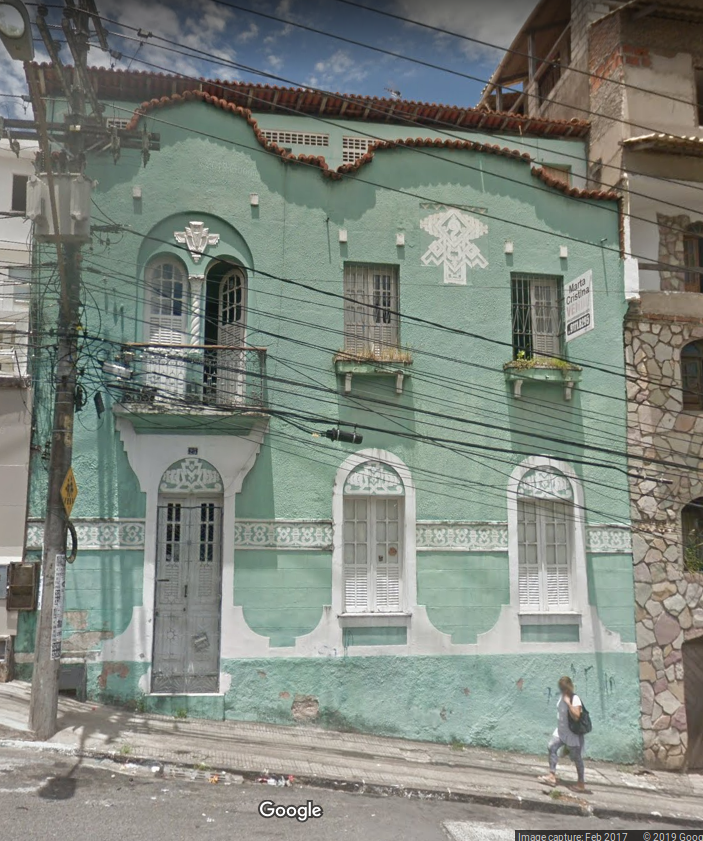
\includegraphics[width=1\textwidth]{8-anexos/plantas/01-1distrito/12-gales/ladeiradosgales-edmundoguimaraes-casa2017.jpg}{\footnotesize \par \textbf{Fonte:} Google Maps. }
\label{fig:edmundoguimaraes2017}
\end{figure}
}

% ---
\chapter{Plantas selecionadas de obras na Boa Vista, no Engenho Velho de Brotas e vizinhança}
% ---

%\afterpage{
%\begin{a3paisagem}
%\begin{figure}[!h]
%\centering
%\caption{}
%\includegraphics[height=0.9\textheight]{8-anexos/plantas/09-amaralinapituba/19-amaralina/.jpg}{\footnotesize \par \textbf{Fonte:} \textbf{BR BAAHMS}, Fundo ``Intendência'', Série ``Processos de Licenciamento de Reforma e Ampliação de Edificações'', Subsérie ``Requerimentos e Plantas -- Brotas'', caixa 19}
%\label{fig:}
%\end{figure}
%\end{a3paisagem}
%}

% ---
\chapter{Plantas selecionadas de obras na Estrada de Brotas e vizinhança}
% ---


%\afterpage{
%\begin{a3paisagem}
%\begin{figure}[!h]
%\centering
%\caption{}
%\includegraphics[height=0.9\textheight]{8-anexos/plantas/09-amaralinapituba/19-amaralina/.jpg}{\footnotesize \par \textbf{Fonte:} \textbf{BR BAAHMS}, Fundo ``Intendência'', Série ``Processos de Licenciamento de Reforma e Ampliação de Edificações'', Subsérie ``Requerimentos e Plantas -- Brotas'', caixa 19}
%\label{fig:}
%\end{figure}
%\end{a3paisagem}
%}

% ---
\chapter{Plantas selecionadas de obras na Estrada Dois de Julho e vizinhança}
% ---

%\afterpage{
%\begin{a3paisagem}
%\begin{figure}[!h]
%\centering
%\caption{}
%\includegraphics[height=0.9\textheight]{8-anexos/plantas/09-amaralinapituba/19-amaralina/.jpg}{\footnotesize \par \textbf{Fonte:} \textbf{BR BAAHMS}, Fundo ``Intendência'', Série ``Processos de Licenciamento de Reforma e Ampliação de Edificações'', Subsérie ``Requerimentos e Plantas -- Brotas'', caixa 19}
%\label{fig:}
%\end{figure}
%\end{a3paisagem}
%}

% ---
\chapter{Plantas selecionadas de obras na Mariquita e vizinhança}
% ---

% ---
% 01. Casa de Theodomiro José Veríssimo, na rua do Céu
% ---

\afterpage{
\begin{a3paisagem}
\begin{figure}[!h]
\centering
\caption{Planta para construcção de uma casa que Bernardo Martins da Silva pretende construir no terreno baldio sito a rua Direita da Mariquita ao Rio Vermelho (1900)}
\includegraphics[width=1\textwidth]{8-anexos/plantas/05-mariquita/06-mariquita/1900-bernardomartinsdasilva.jpg}{\footnotesize \par \textbf{Fonte:} \textbf{BR BAAHMS}, Fundo ``Intendência'', Série ``Processos de Licenciamento de Reforma e Ampliação de Edificações'', Subsérie ``Requerimentos e Plantas -- Brotas'', caixa 06. \par Projeto de desenhista e arquiteto/engenheiro desconhecidos. Casas de veraneio como esta foram comuns na rua Direita da Mariquita. }
\label{fig:1900-bernardomartinsdasilva}
\end{figure}
\end{a3paisagem}
}

% ---
% 02. Casa de Theodomiro José Veríssimo, na rua do Céu
% ---

\afterpage{
\begin{figure}[!h]
\centering
\caption{Projecto para a construcção de uma casa de taipa que Theodomiro José Verissimo pretende fazer na rua do Céo no Rio Vermelho districto de Brotas (1906)}
\includegraphics[width=1\textwidth]{8-anexos/plantas/05-mariquita/03-ruadoceu/theodomirojoseverissimo-1906.jpg}{\footnotesize \par \textbf{Fonte:} \textbf{BR BAAHMS}, Fundo ``Intendência'', Série ``Processos de Licenciamento de Reforma e Ampliação de Edificações'', Subsérie ``Requerimentos e Plantas -- Brotas'', caixa 03. \par Projeto de Custódio Bandeira. Casas de taipa ainda eram toleradas pela Diretoria de Obras na primeira década do século XIX. Mesmo o desenhista ``relaxou'' e não apresentou as medidas de todos os cômodos. }
\label{fig:theodomirojoseverissimo-1906}
\end{figure}
}

% ---
% 03. Casa de Prediliano Pitta, na rua do Lucaia
% ---

\afterpage{
\begin{figure}[!h]
\centering
\caption{Projecto para a construcção de uma casa em terreno baldio, sito à Lucaia freguesia de Brotas, pertencente ao Snr. Prediliano Pereira Pitta (1911)}
\includegraphics[width=1\textwidth]{8-anexos/plantas/05-mariquita/06-lucaia/predilianopitta-1911.jpg}{\footnotesize \par \textbf{Fonte:} \textbf{BR BAAHMS}, Fundo ``Intendência'', Série ``Processos de Licenciamento de Reforma e Ampliação de Edificações'', Subsérie ``Requerimentos e Plantas -- Brotas'', caixa 06. \par Não há assinatura de desenhista ou engenheiro/arquiteto, mas a caligrafia é de Rosalvo Celestino dos Santos. }
\label{fig:predilianopitta-1911}
\end{figure}
}


% ---
% 04. Casa de Luiz Lucas da Costa, na rua da Fonte do Boi
% ---

\afterpage{
\begin{a3paisagem}
\begin{figure}[!h]
\centering
\caption{Projecto para construcção de uma cosinha, varanda, banheiro, latrina e platibanda, em um predio sito a Fonte do Boi no Rio Vermelho districto de Brotas, pertencente ao Sr. Luiz Lucas da Costa (1912)}
\includegraphics[height=0.9\textheight]{8-anexos/plantas/05-mariquita/06-fontedoboi/luizlucasdacosta-1912.jpg}{\footnotesize \par \textbf{Fonte:} \textbf{BR BAAHMS}, Fundo ``Intendência'', Série ``Processos de Licenciamento de Reforma e Ampliação de Edificações'', Subsérie ``Requerimentos e Plantas -- Brotas'', caixa 06. \par Na Mariquita os pedidos de reforma predominaram sobre as construções. Este é um dos poucos projetos em que a fachada original foi desenhada em separado, permitindo perceber as alterações. A casa aliás é pequena: o maior dos cômodos tem 9,79$m^{2}$ e o menor, 6,97$m^{2}$. }
\label{fig:luizlucasdacosta-1912}
\end{figure}
\end{a3paisagem}
}

% ---
% 05. Casa de Manoel Affonso Vianna, na Fonte do Boi
% ---

\afterpage{
\begin{figure}[!h]
\centering
\caption{Projecto de construcção --- propriedade do sr. Manoel Affonso Vianna --- Fonte do Boi (Rio Vermelho) (1913)}
\includegraphics[width=1\textwidth]{8-anexos/plantas/05-mariquita/06-fontedoboi/manoelvianna-1915.jpg}{\footnotesize \par \textbf{Fonte:} \textbf{BR BAAHMS}, Fundo ``Intendência'', Série ``Processos de Licenciamento de Reforma e Ampliação de Edificações'', Subsérie ``Requerimentos e Plantas -- Brotas'', caixa 06. \par Projeto de Humberto Badollato. }
\label{fig:manoelvianna-1915}
\end{figure}
}

% ---
% 06. Casa de Adolpho Moreira, na rua Direita da Mariquita
% ---

\afterpage{
\begin{a3paisagem}
\begin{figure}[!h]
\centering
\caption{Projecto para a reconstrucção da casa à Mariquita, Rio Vermelho, do Snr. Adolpho Moreira (1913)}
\includegraphics[width=0.9\textwidth]{8-anexos/plantas/05-mariquita/06-mariquita/1913-adolphomoreira.jpg}{\footnotesize \par \textbf{Fonte:} \textbf{BR BAAHMS}, Fundo ``Intendência'', Série ``Processos de Licenciamento de Reforma e Ampliação de Edificações'', Subsérie ``Requerimentos e Plantas -- Brotas'', caixa 06. }
\label{fig:1913-adolphomoreira.jpg}
\end{figure}
\end{a3paisagem}
}

% ---
% 07. Padaria de Domingos de Oliveira Reis, na Mariquita
% ---

\afterpage{
\begin{a3paisagem}
\begin{figure}[!h]
\centering
\caption{Rrojecto para a construcção de uma casa e forno de padaria, à rua da Mariquita, Rio Vermelho (1914)}
\includegraphics[height=0.9\textheight]{8-anexos/plantas/05-mariquita/06-mariquita/1914-domingosdeoliveirareis.jpg}{\footnotesize \par \textbf{Fonte:} \textbf{BR BAAHMS}, Fundo ``Intendência'', Série ``Processos de Licenciamento de Reforma e Ampliação de Edificações'', Subsérie ``Requerimentos e Plantas -- Brotas'', caixa 06. \par Projeto de Arthur Santos. O mesmo proprietário tinha uma casa de térreo e primeiro pavimento na Mariquita, vizinha à padaria.}
\label{fig:1914-domingosdeoliveirareis}
\end{figure}
\end{a3paisagem}
}

% ---
% 08. Casa de Maria Zifirina da Conceição
% ---

\afterpage{
\begin{a3paisagem}
\begin{figure}[!h]
\centering
\caption{Progeto de um predio a construir-se na Pedrinha de propriedade da Exma. Snra. D. Maria Zefirina da Conceição (1918)}
\includegraphics[width=1\textwidth]{8-anexos/plantas/05-mariquita/23-pedrinhas/1918-mariazifirinadaconceicao.jpg}{\footnotesize \par \textbf{Fonte:} \textbf{BR BAAHMS}, Fundo ``Intendência'', Série ``Processos de Licenciamento de Reforma e Ampliação de Edificações'', Subsérie ``Requerimentos e Plantas -- Brotas'', caixa 23. \par Projeto de José Portella Passos. Esta casa chama a atenção pelo número de quartos: \textit{oito}, variando entre 7,92$m^{2}$ até os 14,91$m^{2}$. }
\label{fig:1918-mariazifirinadaconceicao}
\end{figure}
\end{a3paisagem}
}

% ---
% 09. Casa de Aurelio Gonçalves Cal
% ---

\afterpage{
\begin{a3paisagem}
\begin{figure}[!h]
\centering
\caption{Representação da casa de nº 30 sita a rua direita da Mariquita, ao Rio Vermelho, com projecto de remodelação de sua fachada e de um pequeno pavimento (1922)}
\includegraphics[height=0.9\textheight]{8-anexos/plantas/05-mariquita/06-mariquita/1922-aureliogoncalvescal.jpg}{\footnotesize \par \textbf{Fonte:} \textbf{BR BAAHMS}, Fundo ``Intendência'', Série ``Processos de Licenciamento de Reforma e Ampliação de Edificações'', Subsérie ``Requerimentos e Plantas -- Brotas'', caixa 06. \par Projeto de Alfredo Vieira de Almeida. Esta casa destaca-se por ter \textit{seis} quartos no primeiro pavimento, e outros \textit{sete} no pavimento a construir, com cerca de 10$m^{2}$ cada.}
\label{fig:1922-aureliogoncalvescal.jpg}
\end{figure}
\end{a3paisagem}
}

% ---
\chapter{Plantas selecionadas de obras no Matatu Grande, Matatu Pequeno, Quinta das Beatas e vizinhança}
% ---



%\afterpage{
%\begin{a3paisagem}
%\begin{figure}[!h]
%\centering
%\caption{}
%\includegraphics[height=0.9\textheight]{8-anexos/plantas/09-amaralinapituba/19-amaralina/.jpg}{\footnotesize \par \textbf{Fonte:} \textbf{BR BAAHMS}, Fundo ``Intendência'', Série ``Processos de Licenciamento de Reforma e Ampliação de Edificações'', Subsérie ``Requerimentos e Plantas -- Brotas'', caixa 19}
%\label{fig:}
%\end{figure}
%\end{a3paisagem}
%}

% ---
\chapter{Plantas selecionadas de obras no Acupe e vizinhança}
% ---




%\afterpage{
%\begin{a3paisagem}
%\begin{figure}[!h]
%\centering
%\caption{}
%\includegraphics[height=0.9\textheight]{8-anexos/plantas/09-amaralinapituba/19-amaralina/.jpg}{\footnotesize \par \textbf{Fonte:} \textbf{BR BAAHMS}, Fundo ``Intendência'', Série ``Processos de Licenciamento de Reforma e Ampliação de Edificações'', Subsérie ``Requerimentos e Plantas -- Brotas'', caixa 19}
%\label{fig:}
%\end{figure}
%\end{a3paisagem}
%}

% ---
\chapter{Plantas selecionadas de obras nas antigas fazendas Alagoa, Amaralina, Santa Cruz, Ubarana e Pituba}\label{cap:anexosamaralina}
% ---



%\afterpage{
%\begin{a3paisagem}
%\begin{figure}[!h]
%\centering
%\caption{}
%\includegraphics[width=\textwidth]{8-anexos/plantas/09-amaralinapituba/19-amaralina/.jpg}{\footnotesize \par \textbf{Fonte:} \textbf{BR BAAHMS}, Fundo ``Intendência'', Série ``Processos de Licenciamento de Reforma e Ampliação de Edificações'', Subsérie ``Requerimentos e Plantas -- Brotas'', caixa 19}
%\label{fig:}
%\end{figure}
%\end{a3paisagem}
%}

\afterpage{
\begin{a3paisagem}
\begin{figure}[!h]
\centering
\caption{Propriedade de A. Saffrey, architecto, Amaralina. Lote 116 da planta geral da cidade d'Amaralina (1915). Projeto de A. Saffrey.}
\includegraphics[height=0.9\textheight]{8-anexos/plantas/09-amaralinapituba/19-amaralina/dsc04777.jpg}{\footnotesize \par \textbf{Fonte:} \textbf{BR BAAHMS}, Fundo ``Intendência'', Série ``Processos de Licenciamento de Reforma e Ampliação de Edificações'', Subsérie ``Requerimentos e Plantas -- Brotas'', caixa 19.}
\label{fig:dsc04777}
\end{figure}
\end{a3paisagem}
}

\afterpage{
\begin{a3paisagem}
\begin{figure}[!h]
\centering
\caption{Projeto de uma casa em Amaralina de D. Lydia Dewald (1915). Desenho de Ciro Spínola, engenheiro desconhecido.}
\includegraphics[height=0.9\textheight]{8-anexos/plantas/09-amaralinapituba/19-amaralina/DSC04783.jpg}{\footnotesize \par \textbf{Fonte:} \textbf{BR BAAHMS}, Fundo ``Intendência'', Série ``Processos de Licenciamento de Reforma e Ampliação de Edificações'', Subsérie ``Requerimentos e Plantas -- Brotas'', caixa 19.}
\label{fig:DSC04783}
\end{figure}
\end{a3paisagem}
}

\afterpage{
\begin{a3paisagem}
\begin{figure}[!h]
\centering
\caption{Projecto da casa que o Ilmº. Snr. José Cardozo da Silva pretende construir em seu terreno, sito à Ubarana, no districto de Brotas (1915). Projeto de Archimedes Marques.}
\includegraphics[height=0.9\textheight]{8-anexos/plantas/09-amaralinapituba/19-amaralina/dsc04791.jpg}{\footnotesize \par \textbf{Fonte:} \textbf{BR BAAHMS}, Fundo ``Intendência'', Série ``Processos de Licenciamento de Reforma e Ampliação de Edificações'', Subsérie ``Requerimentos e Plantas -- Brotas'', caixa 19}
\label{fig:dsc04791}
\end{figure}
\end{a3paisagem}
}

\afterpage{
\begin{a3paisagem}
\begin{figure}[!h]
\centering
\caption{Projecto de uma casa que o sr. Chehadi E. Kraycheti quer construir em Amaralina (1923). Projeto de Eurico da Costa Coutinho.}
\includegraphics[width=\textwidth]{8-anexos/plantas/09-amaralinapituba/19-amaralina/dsc4805.jpg}{\footnotesize \par \textbf{Fonte:} \textbf{BR BAAHMS}, Fundo ``Intendência'', Série ``Processos de Licenciamento de Reforma e Ampliação de Edificações'', Subsérie ``Requerimentos e Plantas -- Brotas'', caixa 19}
\label{fig:dsc4805}
\end{figure}
\end{a3paisagem}
}

\afterpage{
\begin{a3paisagem}
\begin{figure}[!h]
\centering
\caption{Projecto para construção de oito casas à Amaralina, primeira parte (1925). Projeto de Pedro Jayme David.}
\includegraphics[height=0.9\textheight]{8-anexos/plantas/09-amaralinapituba/19-amaralina/dsc04810.jpg}{\footnotesize \par \textbf{Fonte:} \textbf{BR BAAHMS}, Fundo ``Intendência'', Série ``Processos de Licenciamento de Reforma e Ampliação de Edificações'', Subsérie ``Requerimentos e Plantas -- Brotas'', caixa 19}
\label{fig:dsc04810}
\end{figure}
\end{a3paisagem}
}

\afterpage{
\begin{a3paisagem}
\begin{figure}[!h]
\centering
\caption{Projecto para construção de oito casas à Amaralina, segunda parte (1925). Projeto de Pedro Jayme David.}
\includegraphics[width=\textwidth]{8-anexos/plantas/09-amaralinapituba/19-amaralina/dsc04809.jpg}{\footnotesize \par \textbf{Fonte:} \textbf{BR BAAHMS}, Fundo ``Intendência'', Série ``Processos de Licenciamento de Reforma e Ampliação de Edificações'', Subsérie ``Requerimentos e Plantas -- Brotas'', caixa 19}
\label{fig:dsc04809}
\end{figure}
\end{a3paisagem}
}

\afterpage{
\begin{a3paisagem}
\begin{figure}[!h]
\centering
\caption{Projecto para construcção do predio sito na Amaralina, propriedade do Ilmº Snr. João da Cunha Freire, primeira parte (1925). Projeto de Rossi Baptista.}
\includegraphics[height=0.9\textheight]{8-anexos/plantas/09-amaralinapituba/19-amaralina/dsc04813.jpg}{\footnotesize \par \textbf{Fonte:} \textbf{BR BAAHMS}, Fundo ``Intendência'', Série ``Processos de Licenciamento de Reforma e Ampliação de Edificações'', Subsérie ``Requerimentos e Plantas -- Brotas'', caixa 19}
\label{fig:dsc04813}
\end{figure}
\end{a3paisagem}
}

\afterpage{
\begin{a3paisagem}
\begin{figure}[!h]
\centering
\caption{Projecto para construcção do predio sito na Amaralina, propriedade do Ilmº Snr. João da Cunha Freire, segunda parte (1925). Projeto de Rossi Baptista.}
\includegraphics[width=\textwidth]{8-anexos/plantas/09-amaralinapituba/19-amaralina/dsc04814.jpg}{\footnotesize \par \textbf{Fonte:} \textbf{BR BAAHMS}, Fundo ``Intendência'', Série ``Processos de Licenciamento de Reforma e Ampliação de Edificações'', Subsérie ``Requerimentos e Plantas -- Brotas'', caixa 19}
\label{fig:dsc04814}
\end{figure}
\end{a3paisagem}
}

% ---
\chapter{Documentos selecionados}
% ---

\afterpage{
\begin{figure}[!h]
\centering
\caption{Orçamento para construcção de uma capella no Cemiterio de Brotas, incluindo a ampliação da mesma ordenada pelo Exmº. Snr. Dr. Intendente (1928)}
\includegraphics[width=\textwidth]{8-anexos/documentos/tabela-custos-construcao-capela-cemiterio.jpg}{\footnotesize \par \textbf{Fonte:} \textbf{BR BAAHMS}, Fundo ``Intendência'', Série ``Processos de Licenciamento de Reforma e Ampliação de Edificações'', Subsérie ``Requerimentos e Plantas -- Brotas'', caixa 11, proc. 3412 fls. 34. \par Com esta tabela foi possível ter uma ideia do custo da construção civil em Salvador em 1928.}
\label{fig:tabelaconstru}
\end{figure}
}

% \afterpage{
% \begin{a3paisagem}
% \begin{figure}[!h]
% \centering
% \caption{}
% \includegraphics[width=\textwidth]{8-anexos/plantas/09-amaralinapituba/19-amaralina/.jpg}{\footnotesize \par \textbf{Fonte:} \textbf{BR BAAHMS}, Fundo ``Intendência'', Série ``Processos de Licenciamento de Reforma e Ampliação de Edificações'', Subsérie ``Requerimentos e Plantas -- Brotas'', caixa 19}
% \label{fig:}
% \end{figure}
% \end{a3paisagem}
% }

% ---
\chapter{``A Boa Vista'', por Castro Alves}\label{cap:boavista}
% ---

% \poemtitle{A Boa Vista}
\settowidth{\versewidth}{}

\begin{flushright}
\textit{Sonha, poeta, sonha! Aqui sentado \\
No tosco assento da janela antiga,\\
Apóias sobre a mão a face pálida,\\
Sorrindo — dos amores à cantiga.}\\
Álvares de Azevedo
\end{flushright}

\begin{verse}
Era uma tarde triste, mas límpida e suave... \\
Eu — pálido poeta — seguia triste e grave \\
A estrada, que conduz ao campo solitário, \\
Como um filho, que volta ao paternal sacrário, \\
\end{verse}

\begin{verse}
E ao longe abandonando o múrmur da cidade \\
— Som vago, que gagueja em meio à imensidade, — \\
No drama do crepúsculo eu escutava atento \\
A surdina da tarde ao sol, que morre lento. \\
\end{verse}

\begin{verse}
A poeira da estrada meu passo levantava, \\
Porém minh'alma ardente no céu azul marchava \\
E os astros sacudia no vôo violento \\
— Poeira, que dormia no chão do firmamento. \\
\end{verse}

\begin{verse}
A pávida andorinha, que o vendaval fustiga, \\
Procura os coruchéus da catedral antiga. \\
Eu — andorinha entregue aos vendavais do inverno, \\
Ia seguindo triste p'ra o velho lar paterno. \\
\end{verse}

\begin{verse}
Como a águia, que do ninho talhado no rochedo \\
Ergue o pescoço calvo por cima do fraguedo, \\
— (P'ra ver no céu a nuvem, que espuma o firmamento, \\
E o mar, — corcel que espuma ao látego do vento...) \\
Longe o feudal castelo levanta a antiga torre, \\
Que aos raios do poente brilhante sol escorre! \\
Ei-lo soberbo e calmo o abutre de granito \\
Mergulhando o pescoço no seio do infinito \\
E lá de cima olhando com seus clarões vermelhos \\
Os tetos, que a seus pés parecem de joelhos!... \\
\end{verse}

\begin{verse}
Não! Minha velha torre! Oh! atalaia antiga, \\
Tu olhas esperando alguma face amiga, \\
E perguntas talvez ao vento, que em ti chora: \\
``Por que não volta mais o meu senhor d'outrora? \\
Por que não vem sentar-se no banco do terreiro \\
Ouvir das criancinhas o riso feiticeiro, \\
E pensando no lar, na ciência, nos pobres \\
Abrigar nesta sombra seus pensamentos nobres? \\
\end{verse}

\begin{verse}
Onde estão as crianças — grupo alegre e risonho \\
— Que escondiam-se atrás do cipreste tristonho... \\
\end{verse}

\begin{verse}
Ou que enforcaram rindo um feio Pulchinello, \\
Enquanto a doce Mãe, que é toda amor, desvelo \\
Ralha com um rir divino o grupo folgazão, \\
Que vem correndo alegre beijar-lhe a branca mão?...'' \\
\end{verse}

\begin{verse}
É nisto que tu cismas, ó torre abandonada, \\
Vendo deserto o parque e solitária a estrada. \\
No entanto eu — estrangeiro, que tu já não conheces — \\
No limiar de joelhos só tenho pranto e preces. \\
\end{verse}

\begin{verse}
Oh! deixem-me chorar!... Meu lar... meu doce ninho! \\
Abre a vetusta grade ao filho teu mesquinho! \\
Passado — mar imenso!... inunda-me em fragrância! \\
Eu não quero lauréis, quero as rosas da infância. \\
\end{verse}

\begin{verse}
Ai! Minha triste fronte, aonde as multidões \\
Lançaram misturadas glórias e maldições... \\
Acalenta em teu seio, ó solidão sagrada! \\
Deixa est'alma chorar em teu ombro encostada! \\
\end{verse}

\begin{verse}
Meu lar está deserto... Um velho cão de guarda \\
Veio saltando a custo roçar-me a testa parda, \\
Lamber-me após os dedos, porém a sós consigo \\
Rusgando com o direito, que tem um velho amigo... \\
Como tudo mudou-se!... O jardim 'stá inculto \\
As roseiras morreram do vento ao rijo insulto... \\
A erva inunda a terra; o musgo trepa os muros \\
A ortiga silvestre enrola em nós impuros \\
Uma estátua caída, em cuja mão nevada \\
A aranha estende ao sol a teia delicada!... \\
Mergulho os pés nas plantas selvagens, espalmadas, \\
As borboletas fogem-me em lúcidas manadas... \\
E ouvindo-me as passadas tristonhas, taciturnas, \\
Os grilos, que cantavam, calaram-se nas furnas... \\
\end{verse}

\begin{verse}
Oh! jardim solitário! Relíquia do passado! \\
Minh'alma, como tu, é um parque arruinado! \\
Morreram-me no seio as rosas em fragrância, \\
Veste o pesar os muros dos meus vergéis da infância, \\
\end{verse}

\begin{verse}
A estátua do talento, que pura em mim s'erguia, \\
Jaz hoje — e nela a turba enlaça uma ironia!... \\
Ao menos como tu, lá d'alma num recanto \\
Da casta poesia ainda escuto o canto, \\
— Voz do céu, que consola, se o mundo nos insulta, \\
E na gruta do seio murmura um treno oculta. \\
\end{verse}

\begin{verse}
Entremos!... Quantos ecos na vasta escadaria, \\
Nos longos corredores respondem-me à porfia!... \\
\end{verse}

\begin{verse}
Oh! casa de meus pais!... A um crânio já vazio, \\
Que o hóspede largando deixou calado e frio, \\
Compara-te o estrangeiro — caminhando indiscreto \\
Nestes salões imensos, que abriga o vasto teto. \\
\end{verse}

\begin{verse}
Mas eu no teu vazio — vejo uma multidão \\
Fala-me o teu silêncio — ouço-te a solidão!... \\
Povoam-se estas salas... \\
\end{verse}

\begin{verse}
E eu vejo lentamente \\
No solo resvalarem falando tenuemente \\
Dest'alma e deste seio as sombras venerandas \\
Fantasmas adorados — visões sutis e brandas... \\
\end{verse}

\begin{verse}
Aqui... além... mais longe... por onde eu movo o passo, \\
Como aves, que espantadas arrojam-se ao espaço, \\
Saudades e lembranças s'erguendo — bando alado — \\
Roçam por mim as asas voando p'ra o passado. \\
\end{verse}

\attrib{Boa Vista, 18 de novembro de 1867.}

\end{anexosenv}